\documentclass{report}

\usepackage[utf8]{inputenc}
\usepackage[T1]{fontenc}
\usepackage[francais]{babel}
\usepackage{graphicx}
\usepackage{circuitikz}
\usepackage[squaren, Gray]{SIunits}
\usepackage{sistyle}
\usepackage[autolanguage]{numprint}
\usepackage{pgfplots}
\pgfplotsset{compat=1.9}
\usepackage{amsmath,amssymb,array}
\usepackage[top=2.5cm,bottom=2.5cm,right=2.5cm,left=2.5cm]{geometry}
\usepackage{tabularx}
\DeclareMathOperator{\dist}{d}
\newenvironment{abstract-fr}
{
	\begin{center}
		\textbf{Résumé} \\[0.5cm]
	\end{center}
}
{}

\newenvironment{abstract-en}
{
	\begin{center}
		\textbf{Summary} \\[0.5cm]
	\end{center}
}
{}
% New command pour la modélisation mécanique, tri à effectuer
\newcommand\fv[1]{{\bf #1}} % free vector
\newcommand\fvd[1]{\dot{\bf #1}} % free vector derivated
\newcommand\fvdd[1]{\ddot{\bf #1}} % free vector derivated
\newcommand\fvr[1]{\mathring{\bf #1}} % free vector relatively derivated
\newcommand\fvrr[1]{\overset{\circ\circ}{\bf #1}} % free vector relatively derivated
\newcommand\uv[1]{{\bf\hat{ #1}}} % unit vector
\newcommand\ui{{\bf\hat{I}}} % unit vector I
\newcommand\uj{{\bf\hat{J}}} % unit vector J
\newcommand\uk{{\bf\hat{K}}} % unit vector K
\newcommand\wrt[2]{\ensuremath{\tensor*[_{ #1}]{ #2}{}}} % With Respect To
\newcommand\wtr[3]{\ensuremath{\tensor*[_{ #1}]{ #2}{^{ #3}}}} % With Two Respect
\newcommand\omegaf{{\bm \omega}}
\newcommand\omegafr{\mathring{\bm \omega}}
\newcommand\omegafd{\dot{\bm \omega}}
\newcommand\omegaft{\tilde{\bm \omega}}
\newcommand\omegaftr{\mathring{\tilde{\bm \omega}}}
\newcommand\omegat{\tilde{\omega}}
\newcommand\omegatd{\tilde{\dot{\omega}}}
\newcommand\ine{{\bf I}}
\newcommand\st{{\bf L}}
\newcommand\pst{{\bf M}}
\newcommand\lm{{\bf N}}
\newcommand\am{{\bf H}}
\newcommand\amd{\dot{\am}}
\newcommand\fo{{\bf F}}
\newcommand\po{\mathcal{P}}
\newcommand\xg{\ensuremath{\fv{R}}}
\newcommand\xgd{\ensuremath{\fvd{R}}}
\newcommand\xgdd{\ensuremath{\fvdd{R}}}
\newcommand\dvec[1]{\dot{\vec{ #1}}}
\newcommand\ddvec[1]{\ddot{\vec{ #1}}}
\newcommand\qp{\dot{q}}
\newcommand\dqp{\Delta \dot{q}}
\usepackage{url} 
\usepackage{hyperref}
\hypersetup{
    colorlinks,
    citecolor=black,
    filecolor=black,
    linkcolor=black,
    urlcolor=black
}

\begin{document}

% Page de garde
\begin{titlepage}
\begin{center}

\includegraphics[width=0.15\textwidth]{logo.jpg}~\\[1cm]

\textsc{\LARGE Ecole Polytechnique de Louvain-La-Neuve}\\[1.5cm]

\textsc{\Large FSAB1502 - Projet 2}\\[0.5cm]

% Title
\HRule \\[0.4cm]
{\huge \bfseries Concevoir, réaliser et qualifier un système de haut-parleur\\[0.5cm]}

\HRule \\[1.5cm]

\begin{minipage}{1.0\textwidth}
\begin{flushleft} \large
\emph{Auteurs : } Groupe \numprint{115.3}\\[0.2cm]

\begin{tabular}{lr}
Thibaut \textsc{Cabo} & (\numprint{4353-1300}) \\
Lise \textsc{Céresiat} & (\numprint{1965-1200}) \\
Robin \textsc{Crits} & (\numprint{3236-1300}) \\
Virgile \textsc{Goyens} & (\numprint{8339-1300}) \\
Antoine \textsc{Paris} & (\numprint{3158-1300}) \\
Marie-Charlotte \textsc{Sparenberg} & (\numprint{5408-1300})
\end{tabular}

\end{flushleft}
\end{minipage}

\HRule \\[1.0cm]

\begin{minipage}{1.0\textwidth}
\begin{flushleft} \large
\emph{Tuteur :} \\[0.2cm]
\begin{tabular}{l}
Pr.~Piotr \textsc{Sobieski}
\end{tabular}
\end{flushleft}
\end{minipage}

\vfill

{\large \today}

\end{center}
\end{titlepage}

% Abstract
\documentclass{article}

\usepackage[utf8]{inputenc}
\usepackage[T1]{fontenc}      
\usepackage[francais]{babel}
\usepackage{graphicx}
\usepackage{circuitikz}
\usepackage[squaren, Gray]{SIunits}
\usepackage{sistyle}
\usepackage[autolanguage]{numprint}
\usepackage{pgfplots}
\usepackage{amsmath,amssymb,array}
\usepackage{url} 

% New command pour la modélisation mécanique, tri à effectuer
\newcommand\fv[1]{{\bf #1}} % free vector
\newcommand\fvd[1]{\dot{\bf #1}} % free vector derivated
\newcommand\fvdd[1]{\ddot{\bf #1}} % free vector derivated
\newcommand\fvr[1]{\mathring{\bf #1}} % free vector relatively derivated
\newcommand\fvrr[1]{\overset{\circ\circ}{\bf #1}} % free vector relatively derivated
\newcommand\uv[1]{{\bf\hat{ #1}}} % unit vector
\newcommand\ui{{\bf\hat{I}}} % unit vector I
\newcommand\uj{{\bf\hat{J}}} % unit vector J
\newcommand\uk{{\bf\hat{K}}} % unit vector K
\newcommand\wrt[2]{\ensuremath{\tensor*[_{ #1}]{ #2}{}}} % With Respect To
\newcommand\wtr[3]{\ensuremath{\tensor*[_{ #1}]{ #2}{^{ #3}}}} % With Two Respect
\newcommand\omegaf{{\bm \omega}}
\newcommand\omegafr{\mathring{\bm \omega}}
\newcommand\omegafd{\dot{\bm \omega}}
\newcommand\omegaft{\tilde{\bm \omega}}
\newcommand\omegaftr{\mathring{\tilde{\bm \omega}}}
\newcommand\omegat{\tilde{\omega}}
\newcommand\omegatd{\tilde{\dot{\omega}}}
\newcommand\ine{{\bf I}}
\newcommand\st{{\bf L}}
\newcommand\pst{{\bf M}}
\newcommand\lm{{\bf N}}
\newcommand\am{{\bf H}}
\newcommand\amd{\dot{\am}}
\newcommand\fo{{\bf F}}
\newcommand\po{\mathcal{P}}
\newcommand\xg{\ensuremath{\fv{R}}}
\newcommand\xgd{\ensuremath{\fvd{R}}}
\newcommand\xgdd{\ensuremath{\fvdd{R}}}
\newcommand\dvec[1]{\dot{\vec{ #1}}}
\newcommand\ddvec[1]{\ddot{\vec{ #1}}}
\newcommand\qp{\dot{q}}
\newcommand\dqp{\Delta \dot{q}}

\begin{document}


\begin{abstract-fr}
Le haut-parleur est un outil permettant de transformer un signal électrique en un signal sonore.  Grâce à une bobine fixe, la bobine mobile peut osciller et faire vibrer la membrane à laquelle elle est attachée, ceci crée une onde sonore.
De nombreuses phases de tests ont été effectuées pour obtenir un haut-parleur fonctionnel, malgré les calculs mathématiques nous avons dû faire des hypothèses simplificatrices et donc seuls les vrais tests reflètent la réalité.
Dans ce document, les calculs et les idées nécessaires à a création d’un tel objet sont présentés.  
Notre haut-parleur est capable de produire un son qui a une fréquence entre \SI{500}{\hertz} et \SI{5000}{\hertz}, a une puissance de \SI{2.5}{\watt}, avec une membrane de \SI{0.17}{\meter} de diamètre, une bobine fixe de \numprint{450} spires et une mobile de \numprint{100}. Avec la prise jack qui permet de relier le haut-parleur à un Gsm ou un mp3, nous pouvons obtenir un son réglable en intensité.
\end{abstract-fr}

% Just here to fix rapport_prejury.tex
\end{document}

\documentclass{article}

\usepackage[utf8]{inputenc}
\usepackage[T1]{fontenc}      
\usepackage[francais]{babel}
\usepackage{graphicx}
\usepackage{circuitikz}
\usepackage[squaren, Gray]{SIunits}
\usepackage{sistyle}
\usepackage[autolanguage]{numprint}
\usepackage{pgfplots}
\usepackage{amsmath,amssymb,array}
\usepackage{url} 

% New command pour la modélisation mécanique, tri à effectuer
\newcommand\fv[1]{{\bf #1}} % free vector
\newcommand\fvd[1]{\dot{\bf #1}} % free vector derivated
\newcommand\fvdd[1]{\ddot{\bf #1}} % free vector derivated
\newcommand\fvr[1]{\mathring{\bf #1}} % free vector relatively derivated
\newcommand\fvrr[1]{\overset{\circ\circ}{\bf #1}} % free vector relatively derivated
\newcommand\uv[1]{{\bf\hat{ #1}}} % unit vector
\newcommand\ui{{\bf\hat{I}}} % unit vector I
\newcommand\uj{{\bf\hat{J}}} % unit vector J
\newcommand\uk{{\bf\hat{K}}} % unit vector K
\newcommand\wrt[2]{\ensuremath{\tensor*[_{ #1}]{ #2}{}}} % With Respect To
\newcommand\wtr[3]{\ensuremath{\tensor*[_{ #1}]{ #2}{^{ #3}}}} % With Two Respect
\newcommand\omegaf{{\bm \omega}}
\newcommand\omegafr{\mathring{\bm \omega}}
\newcommand\omegafd{\dot{\bm \omega}}
\newcommand\omegaft{\tilde{\bm \omega}}
\newcommand\omegaftr{\mathring{\tilde{\bm \omega}}}
\newcommand\omegat{\tilde{\omega}}
\newcommand\omegatd{\tilde{\dot{\omega}}}
\newcommand\ine{{\bf I}}
\newcommand\st{{\bf L}}
\newcommand\pst{{\bf M}}
\newcommand\lm{{\bf N}}
\newcommand\am{{\bf H}}
\newcommand\amd{\dot{\am}}
\newcommand\fo{{\bf F}}
\newcommand\po{\mathcal{P}}
\newcommand\xg{\ensuremath{\fv{R}}}
\newcommand\xgd{\ensuremath{\fvd{R}}}
\newcommand\xgdd{\ensuremath{\fvdd{R}}}
\newcommand\dvec[1]{\dot{\vec{ #1}}}
\newcommand\ddvec[1]{\ddot{\vec{ #1}}}
\newcommand\qp{\dot{q}}
\newcommand\dqp{\Delta \dot{q}}

\begin{document}


\begin{abstract-en}

In this course, \textit{Projet 2}, we have been asked to make a loudspeaker that can be connected to a smartphone with a Jack-plug.

To achieve this task, we had to work out to find a way to go through it.
We had to find mathematical and physical modele but the real problem was too tricky for us so we had to make some simpler assumptions.
However, we couldn't make random assumption because the theory had to fit with the test we did in the lab.

In this document, you'll find the necessary calculations and ideas to make such a tool. It also describes some
of our documentary researches.

Even if our loudspeaker doesn't work as well as we wanted, we learned a lot from this challenge. 

Our state of mind is pretty hard to describe: we are disappointed with the actual loudspeaker but quite proud of us for the rest.

\end{abstract-en}

% Just here to fix rapport_prejury.tex
\end{document}


\clearpage
\tableofcontents
\clearpage

\chapter{Introduction}

\documentclass{article}

\usepackage[utf8]{inputenc}
\usepackage[T1]{fontenc}      
\usepackage[francais]{babel}
\usepackage{graphicx}
\usepackage{circuitikz}
\usepackage[squaren, Gray]{SIunits}
\usepackage{sistyle}
\usepackage[autolanguage]{numprint}
\usepackage{pgfplots}
\usepackage{amsmath,amssymb,array}
\usepackage{url} 

% New command pour la modélisation mécanique, tri à effectuer
\newcommand\fv[1]{{\bf #1}} % free vector
\newcommand\fvd[1]{\dot{\bf #1}} % free vector derivated
\newcommand\fvdd[1]{\ddot{\bf #1}} % free vector derivated
\newcommand\fvr[1]{\mathring{\bf #1}} % free vector relatively derivated
\newcommand\fvrr[1]{\overset{\circ\circ}{\bf #1}} % free vector relatively derivated
\newcommand\uv[1]{{\bf\hat{ #1}}} % unit vector
\newcommand\ui{{\bf\hat{I}}} % unit vector I
\newcommand\uj{{\bf\hat{J}}} % unit vector J
\newcommand\uk{{\bf\hat{K}}} % unit vector K
\newcommand\wrt[2]{\ensuremath{\tensor*[_{ #1}]{ #2}{}}} % With Respect To
\newcommand\wtr[3]{\ensuremath{\tensor*[_{ #1}]{ #2}{^{ #3}}}} % With Two Respect
\newcommand\omegaf{{\bm \omega}}
\newcommand\omegafr{\mathring{\bm \omega}}
\newcommand\omegafd{\dot{\bm \omega}}
\newcommand\omegaft{\tilde{\bm \omega}}
\newcommand\omegaftr{\mathring{\tilde{\bm \omega}}}
\newcommand\omegat{\tilde{\omega}}
\newcommand\omegatd{\tilde{\dot{\omega}}}
\newcommand\ine{{\bf I}}
\newcommand\st{{\bf L}}
\newcommand\pst{{\bf M}}
\newcommand\lm{{\bf N}}
\newcommand\am{{\bf H}}
\newcommand\amd{\dot{\am}}
\newcommand\fo{{\bf F}}
\newcommand\po{\mathcal{P}}
\newcommand\xg{\ensuremath{\fv{R}}}
\newcommand\xgd{\ensuremath{\fvd{R}}}
\newcommand\xgdd{\ensuremath{\fvdd{R}}}
\newcommand\dvec[1]{\dot{\vec{ #1}}}
\newcommand\ddvec[1]{\ddot{\vec{ #1}}}
\newcommand\qp{\dot{q}}
\newcommand\dqp{\Delta \dot{q}}

\begin{document}


% L'objectif du projet + les spécifications attendues + cahier des charges (ref)
Dans le cadre du cours \textit{Projet 2} du deuxième quadrimestre, notre groupe a été amené à 
concevoir un haut-parleur connectable, via une prise Jack \unit{3.5}{\milli\meter}, à un 
GSM ou un MP3 (les contraintes et spécifications sont détaillées dans l'annexe ''Cahier des charges''). 
En plus de cela, notre haut-parleur doit permette un règlage du volume, des graves
et des aigus. Un autre objectif du projet est d'apprendre un travailler et à s'organiser \textit{en groupe}, 
comme le font tous les jours les ingénieurs.

% L'organisation du rapport
Ce rapport s'articule principalement en deux grands chapitres. Le premier
rassemble les différentes étapes de modélisations mathématiques
et physiques de composants du haut-parleur. Dans ce chapitre, nous 
commencerons par une vue générale du haut-parleur qui nous
permettra d'introduire les concepts physiques clés. Nous continuerons
ensuite par la modélisation des filtres passe-bas, passe-haut et passe bande.
Après cela, nous nous attarderons  sur le dimensionnement de l'électroaimant et
de la bobine mobile pour enfin terminer par la modélisation mécanique de la bobine
mobile.

Le deuxième chapitre contient quant à lui la synthèse des recherches documentaires
effectuées. Ces recherches portent sur deux sujets liés à notre haut-parleur. Le premier
concerne plutôt l'acoustique, il s'agit de la 
distorsion harmonique. Le deuxième quant à lui concerne un concept lié au circuit électrique qui
compose notre haut-parleur, il s'agit du principe de la contre-réaction.

% Description générale du système
Un haut-parleur est un outil permettant de transformer un signal 
électrique en un son. Grâce à un électro-aimant constituée d'une 
bobine fixe dans laquelle passe du courant, une bobine mobile 
oscille et fait vibrer la membrane à laquelle elle est attachée. 
Cette oscillation, qui dépend de la fréquence du signal électrique, 
crée une onde sonore.

Dans notre haut-parleur nous pouvons retrouver la membrane, la plaquette électrique, l
a bobine fixe et mobile, les sources de tension et le caisson.  Chaque partie a 
une particularité et ensemble, le haut-parleur peut remplir sa fonction.  Deux sources
de tension sont relié à la plaquette qui est elle-même relié au GSM d’une part et à 
la bobine mobile d’autre part.  Une autre source de tension permet à la bobine fixe de 
créer un champ magnétique constant.  La fréquence émise par le GSM permet à la bobine 
mobile de bouger selon la musique et la membrane vibre pour émettre le son souhaité.

% Just here to fix rapport_prejury.tex
\end{document}

\chapter{Fonctionnement du haut-parleur}

\documentclass{article}

\usepackage[utf8]{inputenc}
\usepackage[T1]{fontenc}      
\usepackage[francais]{babel}
\usepackage{graphicx}
\usepackage{circuitikz}
\usepackage[squaren, Gray]{SIunits}
\usepackage{sistyle}
\usepackage[autolanguage]{numprint}
\usepackage{pgfplots}
\usepackage{amsmath,amssymb,array}
\usepackage{url} 

% New command pour la modélisation mécanique, tri à effectuer
\newcommand\fv[1]{{\bf #1}} % free vector
\newcommand\fvd[1]{\dot{\bf #1}} % free vector derivated
\newcommand\fvdd[1]{\ddot{\bf #1}} % free vector derivated
\newcommand\fvr[1]{\mathring{\bf #1}} % free vector relatively derivated
\newcommand\fvrr[1]{\overset{\circ\circ}{\bf #1}} % free vector relatively derivated
\newcommand\uv[1]{{\bf\hat{ #1}}} % unit vector
\newcommand\ui{{\bf\hat{I}}} % unit vector I
\newcommand\uj{{\bf\hat{J}}} % unit vector J
\newcommand\uk{{\bf\hat{K}}} % unit vector K
\newcommand\wrt[2]{\ensuremath{\tensor*[_{ #1}]{ #2}{}}} % With Respect To
\newcommand\wtr[3]{\ensuremath{\tensor*[_{ #1}]{ #2}{^{ #3}}}} % With Two Respect
\newcommand\omegaf{{\bm \omega}}
\newcommand\omegafr{\mathring{\bm \omega}}
\newcommand\omegafd{\dot{\bm \omega}}
\newcommand\omegaft{\tilde{\bm \omega}}
\newcommand\omegaftr{\mathring{\tilde{\bm \omega}}}
\newcommand\omegat{\tilde{\omega}}
\newcommand\omegatd{\tilde{\dot{\omega}}}
\newcommand\ine{{\bf I}}
\newcommand\st{{\bf L}}
\newcommand\pst{{\bf M}}
\newcommand\lm{{\bf N}}
\newcommand\am{{\bf H}}
\newcommand\amd{\dot{\am}}
\newcommand\fo{{\bf F}}
\newcommand\po{\mathcal{P}}
\newcommand\xg{\ensuremath{\fv{R}}}
\newcommand\xgd{\ensuremath{\fvd{R}}}
\newcommand\xgdd{\ensuremath{\fvdd{R}}}
\newcommand\dvec[1]{\dot{\vec{ #1}}}
\newcommand\ddvec[1]{\ddot{\vec{ #1}}}
\newcommand\qp{\dot{q}}
\newcommand\dqp{\Delta \dot{q}}

\begin{document}


\section{Fonctionnement général}
% Description générale du système + concepts physiques clés
Notre haut-parleur peut être représenté schématiquement comme sur la Figure \ref{block-diagram-hp}.

% Schéma montrant le bonne compréhension du système
\begin{figure}[!htb]
	\centering
	\includegraphics[scale=0.9]{schema_fonctionnel.png}
	\caption{Schéma fonctionnel du haut-parleur.}
	\label{block-diagram-hp}
\end{figure}

Le GSM ou le MP3 va dans un premier temps envoyer un signal audio via le câble Jack au circuit
imprimé; par la suite nous qualifierons ce signal de \textit{brut}. Le circuit imprimé permet
quant à lui de modifier ce signal brut de plusieurs façon : 

\begin{itemize}
	\item En règlant le volume, c'est-à-dire en modifiant l'amplitude du signal audio ;
	\item En règlant les graves et les aigus, c'est-à-dire en atténuant les basses fréquences
	(rôle du filtre passe-haut, circuit CR) ou les hautes
	fréquences (rôle du filtre passe-bas, circuit RC). Il s'agit du rôle des filtres passe-bas 
	et passe-haut qui,  combinés, forment un filtre passe-bande ;
	\item En amplifiant le signal : c'est le rôle de l'amplificateur audio du circuit.
\end{itemize}

À la sortie du circuit imprimé, le signal est alors \textit{filtré} et \textit{amplifié}.
Ce signal traité ira ensuite alimenter en courant la bobine mobile. Cette 
dernière intercepte un champ magnétique constant, noté $B$, produit par l'électroaimant.
L'électroaimant est constitué de fines lamelles de matériau magnétique en forme de ''E'' 
empilées les unes sur les autres. La perméabilité magnétique élevée de ce matériau
($\mu_r \approx \ 1600$) permet de créer un champ magnétique plus fort. Autour de la branche
centrale du ''E'' est enroulé du fil de cuivre, formant ainsi une bobine.
% Premier concept physique, loi d'Ampère
Le champ magnétique $B$ produit par l'électroaimant dans l'entrefer peut être calculer par la 
loi d'\textsc{Ampère} :

$$\vec{B} = \mu_0\mu_r\frac{NI}{e}$$

Où $N$ est le nombre de spires, $I$ le courant traversant la bobine et $e$ la largeur de 
l'entefer.

% Deuxième concept physique, force de Laplace
La bobine mobile subit donc une force de \textsc{Laplace} dont l'expression est :

$$\vec{F} = i(t)\vec{L}\times{\vec{B}}$$ 

Où $L$ est la longueur du fil et$i(t)$ le courant le traversant. Cette force est proportionnelle
au courant traversant
la bobine mobile. La membrane se déplacera donc de manière cohérente avec le signal audio
et reproduira le son voulu. Enfin, la membrane pourra revenir à sa position d'équilibre
grâce à des attaches qui, à la manière de ressorts, produisent une force de rappel dans la
direction opposée au mouvement de la bobine mobile :

$$\vec{F} = -kx$$ % Troisième concept physique, loi d'Hook

Ou $k$ est la constante de raideur des attaches et $x$ est le déplacement de la bobine mobile
par rapport à sa position d'origine (et donc la compression des attaches).

\paragraph{Remarque}
Une description plus détaillée de chaque composant du circuit électrique est présentée
dans l'annexe ''Analyse séquentielle du circuit''.

% Just here to fix rapport_prejury.tex
\end{document}

\clearpage

\documentclass{article}

\usepackage[utf8]{inputenc}
\usepackage[T1]{fontenc}      
\usepackage[francais]{babel}
\usepackage{graphicx}
\usepackage{circuitikz}
\usepackage[squaren, Gray]{SIunits}
\usepackage{sistyle}
\usepackage[autolanguage]{numprint}
\usepackage{pgfplots}
\usepackage{amsmath,amssymb,array}
\usepackage{url} 

% New command pour la modélisation mécanique, tri à effectuer
\newcommand\fv[1]{{\bf #1}} % free vector
\newcommand\fvd[1]{\dot{\bf #1}} % free vector derivated
\newcommand\fvdd[1]{\ddot{\bf #1}} % free vector derivated
\newcommand\fvr[1]{\mathring{\bf #1}} % free vector relatively derivated
\newcommand\fvrr[1]{\overset{\circ\circ}{\bf #1}} % free vector relatively derivated
\newcommand\uv[1]{{\bf\hat{ #1}}} % unit vector
\newcommand\ui{{\bf\hat{I}}} % unit vector I
\newcommand\uj{{\bf\hat{J}}} % unit vector J
\newcommand\uk{{\bf\hat{K}}} % unit vector K
\newcommand\wrt[2]{\ensuremath{\tensor*[_{ #1}]{ #2}{}}} % With Respect To
\newcommand\wtr[3]{\ensuremath{\tensor*[_{ #1}]{ #2}{^{ #3}}}} % With Two Respect
\newcommand\omegaf{{\bm \omega}}
\newcommand\omegafr{\mathring{\bm \omega}}
\newcommand\omegafd{\dot{\bm \omega}}
\newcommand\omegaft{\tilde{\bm \omega}}
\newcommand\omegaftr{\mathring{\tilde{\bm \omega}}}
\newcommand\omegat{\tilde{\omega}}
\newcommand\omegatd{\tilde{\dot{\omega}}}
\newcommand\ine{{\bf I}}
\newcommand\st{{\bf L}}
\newcommand\pst{{\bf M}}
\newcommand\lm{{\bf N}}
\newcommand\am{{\bf H}}
\newcommand\amd{\dot{\am}}
\newcommand\fo{{\bf F}}
\newcommand\po{\mathcal{P}}
\newcommand\xg{\ensuremath{\fv{R}}}
\newcommand\xgd{\ensuremath{\fvd{R}}}
\newcommand\xgdd{\ensuremath{\fvdd{R}}}
\newcommand\dvec[1]{\dot{\vec{ #1}}}
\newcommand\ddvec[1]{\ddot{\vec{ #1}}}
\newcommand\qp{\dot{q}}
\newcommand\dqp{\Delta \dot{q}}

\begin{document}


\section{Modélisation des filtres passe-haut et passe-bas}
Dans cette section, nous allons expliquer la méthode que nous avons
utiliseé pour trouver une expression analytique de la tension de sortie 
dans un filtre passe-bas, la démarche étant la même pour le filtre passe-haut.

Nous avons en réalité utilisé deux méthodes différentes qui, heureusement, 
aboutissent à la même solution. La première méthode utilise ce que nous
avons appris au premier quadrimestre concernant les équations différentielles.
Cette méthode est plus longue et plus compliquée que la deuxième, c'est pourquoi
nous ne la décrirons pas ici.
La deuxième méthode utilise ce que nous avons appris au deuxième quadrimestre 
concernant les équations différentielles et les complexes. 

\subsection{Le filtre passe-bas}

Soit $V_R$ la tension à travers la résistance $R$, $V_C$ la tension à travers
le condensateur $C$, $V_{in}$ la tension d'entrée et $V_{out}$ la tension de
sortie du filtre.

\begin{figure}[ht!]
	\centering
	\begin{circuitikz}
		\draw (0,0) node[ocirc] (A);
		\draw (0,0) to [R=$R$] (2,0);
		\draw (2,0) to [short] (4,0);
		\draw (4,0) node[ocirc] (C);
		\draw (2,0) to [C=$C$] (2,-2);
		\draw (2,-2) to [short] (4,-2);
		\draw (4,-2) node[ocirc] (D);
		\draw (0,-2) to [short] (2,-2);
		\draw (0,-2) node[ocirc] (B);
		\draw (A) to[open, v=$V_ {in}$] (B);
		\draw (C) to[open, v=$V_{out}$] (D);
	\end{circuitikz}
	\caption{Schéma électrique d'un filtre passe-bas}
	\label{lwp_scheme}
\end{figure}

Sur le circuit ci-dessus (Figure \ref{lwp_scheme}), on peut utiliser la loi des tensions de Kirchhoff :

$$V_{in} = V_R + V_{out}$$

On note $V$ l'amplitude de la tension d'entrée sinusoïdale, $i(t)$ est le courant
en fonction du temps : 

$$V \cdot \cos (\omega t) = R \cdot i(t) + V_C$$

Or, le courant $i(t)$ à travers un condensateur est donné par $C \frac{dV_C}{dt}$, 
l'équation devient alors une équation différentielle en la fonction inconnue $V_C (t)$ :

$$V \cdot \cos (\omega t) = RC\frac{dV_C}{dt}  + V_C$$

On peut réecrire cette équation de la manière suivante, où $y = V_C(t)$ :

$$RCy' + y = V \cdot \cos (\omega t)$$

Cette équation va être la base de la méthode qui suit. On va également utiliser 
la condition initiale suivante :

$$y(0) = 0$$

\subsubsection{Résolution de l'équation différentielle}

On sait que $\cos (\omega t)$ est égale à la partie réelle de l'exponentielle
complexe $e^{\omega i t}$. On réecrit alors l'équation différentielle de la
manière suivante :

$$RCy' + y = V \cdot e^{\omega i t}$$

Comme pour toute équation différentielle linéaire non-homogène, nous allons travailler
en deux étapes :

\paragraph{Recherche de la solution homogène}

Le polynôme caractéristique de l'équation homogène est :

$$RC \cdot x + 1 = 0$$

On a alors $x = \frac{-1}{RC}$ comme racine, et on trouve donc comme solution homogène :

$$y_h(t) = A \cdot e^{\frac{-t}{RC}}$$

Où $A$ est une constante appartenant à l'ensemble des réels. % A confirmer, j'ai un doute.

\paragraph{Recherche de la solution particulière}

La solution particulière qu'on recherche est de la forme :

$$y_p(t) = \alpha \cdot e^{\omega i t}$$

Il nous reste donc à déterminer la constante complexe $\alpha$. Pour ce faire,
nous injectons dans l'équation de départ $y_p(t)$ et sa dérivée première. On
trouve alors :

$$\alpha = \frac{V(1-RC\omega i)}{1+R^2C^2\omega^2}$$

La solution particulière est donc :

$$y_p(t) = \frac{V(1-RC\omega i)}{1+R^2C^2\omega^2} \cdot e^{\omega i t}$$

\paragraph{Solution complète}

La solution finale $y(t)$ est égale à $y_h(t) + y_p(t)$ :

$$y(t) = A \cdot e^{\frac{-t}{RC}} + \frac{V(1-RC\omega i)}{1+R^2C^2\omega^2} \cdot e^{\omega i t}$$

En retransformant ensuite l'exponentielle complexe en sa forme trigonométrique et en ne
gardant que la partie réelle, on trouve :

$$y(t) = V_C(t) = \frac{V(\cos (\omega t) + RC\omega \sin (\omega t))}{1 + \omega^2R^2C^2} + A \cdot e^{\frac{-t}{RC}}$$

\paragraph{Elimination de la constante}

Il ne nous reste plus qu'à éliminer la constante $A$ en utilisant la condition initiale.
On trouve enfin :

$$A = -\frac{V}{1 + \omega^2R^2C^2}$$                         

\paragraph{Conclusion}

La tension de sortie en fonction du temps est donc donnée par :

$$V_{out} = \frac{V}{1 + \omega^2R^2C^2} \cdot (\cos (\omega t) + RC\omega \sin (\omega t) - e^{\frac{-t}{RC}})$$

On peut ensuite réecrire cette formule de manière à faire apparaître
le déphasage de la tension de sortie par rapport à la tension d'entrée. En transformant
$y_p(t)$ en utilisant la notation exponentielle $|z|e^{\phi i}$ d'un couple de la forme 
$a+bi$ et en utilisant ensuite la notation trigonométrique d'une exponentielle complexe,
on trouve, après quelques simplifications et mises en évidence :

$$V_{out} = \frac{V}{\sqrt{1 + R^2\omega^2C^2}}
\left(-\frac{e^{\frac{-t}{RC}}}{\sqrt{1 + R^2\omega^2C^2}} + \cos(\arctan(-RC\omega) + \omega t)\right)$$

On remarque donc que le déphasage entre $V_{out}$ et $V_{in}$ est $-\arctan(RC\omega) = -\arctan(2\pi fRC)$.
Ce déphasage augmente donc linéairement avec $\omega$ et est dû au temps que met le condensateur
à se charger. % A vérifier

\subsubsection{Vérification des résultats}

Une première vérification que l'on peut faire est de vérifier que $V_{out}$ tend vers 0
lorsque $\omega$ tend vers l'infini. C'est bien le cas ici puisqu'on a $\omega^2$ au dénominateur.

On peut ensuite regarder les graphes de $V_{out}$, $V_{in}$ (Figure \ref{lwp_voltages}) et $V_{out} / V_{in}$
(Figure \ref{lwp_ratio}).

\begin{figure}[ht!]
	\centering
	\begin{tikzpicture}[>=stealth]
    \begin{axis}[
        xmin=0,xmax=6,
        ymin=-8,ymax=8,
        axis x line=middle,
        axis y line=middle,
        axis line style=->,
        xlabel={$V$},
        ylabel={$t$},
        ]
				
        \addplot[no marks,black,-] expression[domain=0:6,samples=1000]
						{((7.5)/(sqrt(1 + 1000^2 * 0.00001^2 * 400^2))) * (((-2.718^((-x)/(1000*0.00001)))/(sqrt(1 + 1000^2 * 0.00001^2 * 400^2))) 
						+ cos(atan(-1000*0.00001*400) + 400*x))} 
						node[pos=0.65,anchor=south west]{$$};
						
				\addplot[no marks,blue,-] expression[domain=0:6,samples=1000]
						{7.5 * cos(400 * x)} 
						node[pos=0.65,anchor=south west]{$$}; 

    \end{axis}
	\end{tikzpicture}
	\caption{Graphe de $V_{out}$ (en noir) et $V_{in}$ (en bleu) pour les valeurs suivantes : $V_{max} = \unit{7.5}{\volt}$, $C = \unit{0.00001}{\farad}$,
						$R = \unit{1000}{\ohm}$ et $f = \unit{63.66}{\hertz}$}
	\label{lwp_voltages}
\end{figure}

\begin{figure}[ht!]
	\centering
	\begin{tikzpicture}[>=stealth]
    \begin{axis}[
        xmin=0,xmax=1400,
        ymin=0,ymax=1.2,
        axis x line=middle,
        axis y line=middle,
        axis line style=->,
        xlabel={$f$},
        ylabel={$V_{out} / V_{in}$},
        ]
				
				\addplot[no marks,green,-] expression[domain=0:1400,samples=100]
						% Formule par rapport aux expressions obtenues, un peu décallée
						% {(((7.5)/(sqrt(1 + 100^2 * 0.00001^2 * (2*3.14*x)^2))) * (((-2.718^((-100*0.00001)/(100*0.00001)))/(sqrt(1 + 100^2 * 
						% 0.00001^2 * (2*3.14*x)^2))) + cos(atan(-100*0.00001*2*3.14*x) + 2*3.14*x*100*0.00001)))/(7.5 * cos(2*3.14*x*100*0.00001))}
						{(1 + (2*3.14*x*100*0.00001)^2)^(-0.5)}
						node[pos=0.65,anchor=south west]{$$}; 
    \end{axis}
	\end{tikzpicture}
	\caption{Graphe de $V_{out} / V_{in}$ pour les valeurs suivantes : $R = \unit{100}{\ohm}$ et $C = {\unit{0.0001}{\farad}}$.}
	\label{lwp_ratio}
\end{figure}

\bigbreak

\subsection{Le filtre passe-haut}

Soit $V_R$ la tension à travers la résistance $R$, $V_C$ la tension à travers
le condensateur $C$, $V_{in}$ la tension d'entrée et $V_{out}$ la tension de
sortie du filtre.

\begin{figure}[ht!]
	\centering
	\begin{circuitikz}
		\draw (0,0) node[ocirc] (A);
		\draw (0,0) to [C=$C$] (2,0);
		\draw (2,0) to [short] (4,0);
		\draw (4,0) node[ocirc] (C);
		\draw (2,0) to [R=$R$] (2,-2);
		\draw (2,-2) to [short] (4,-2);
		\draw (4,-2) node[ocirc] (D);
		\draw (0,-2) to [short] (2,-2);
		\draw (0,-2) node[ocirc] (B);
		\draw (A) to[open, v=$V_ {in}$] (B);
		\draw (C) to[open, v=$V_{out}$] (D);
	\end{circuitikz}
	\caption{Schéma électrique d'un filtre passe-haut.}
	\label{hgp_scheme}
\end{figure}

Sur la Figure \ref{hgp_scheme}, la loi des tensions de Kirchhoff donne la même équation que pour le filtre passe-bas :

$$V_{in} = V_R + V_C$$

Cette fois, $V_{out} = V_R$. Or on connait déjà $V_C$ que l'on a calculé dans
le section précédente. On a alors simplement :

$$V_R = V_{in} - V_C$$

$$V_{out} = \frac{V}{\sqrt{1 + R^2\omega^2C^2}}
\left(\frac{e^{\frac{-t}{RC}}}{\sqrt{1 + R^2\omega^2C^2}} - \cos(\arctan(-RC\omega) + \omega t) \right) + \cos(\omega t)$$


Le déphasage reste donc le même que pour le filtre passe-bas.

\subsubsection{Vérification des résultats}

Pour le filtre passe-haut, on va cette fois vérifier que lorsque $\omega$ tend vers 0, on a
$V_{out}$ qui tend vers 0 également. Une fois de plus, c'est bien le cas.

On peut ensuite comparer les graphes de $V_{out}$, $V_{in}$ (Figure \ref{hgp_voltages}) et $V_{out} / V_{in}$
(Figure \ref{hgp_ratio}).

\begin{figure}[ht!]
	\centering
	\begin{tikzpicture}[>=stealth]
    \begin{axis}[
        xmin=0,xmax=6,
        ymin=-8,ymax=8,
        axis x line=middle,
        axis y line=middle,
        axis line style=->,
        xlabel={$V$},
        ylabel={$t$},
        ]
				
        \addplot[no marks,black,-] expression[domain=0:6,samples=1000]
						{(7.5 * cos(100*x)) - ((7.5)/(sqrt(1 + 1000^2 * 0.00001^2 * 100^2))) * (((-2.718^((-x)/(1000*0.00001)))/(sqrt(1 + 1000^2 *
						0.00001^2 * 100^2))) + cos(atan(-1000*0.00001*100) + 100*x))} 
						node[pos=0.65,anchor=south west]{$V_{out}$};
						
				\addplot[no marks,blue,-] expression[domain=0:25,samples=1000]
						{7.5 * cos(100 * x)} 
						node[pos=0.65,anchor=south west]{$V_{in}$}; 
				
    \end{axis}
	\end{tikzpicture}
	\caption{Graphe de $V_{out}$ et $V_{in}$ pour les valeurs suivantes : $V_{max} = \unit{7.5}{\volt}$, $C = \unit{0.00001}{\farad}$,
					$R = \unit{1000}{\ohm}$ et $f = \unit{15.91}{\hertz}$}
	\label{hgp_voltages}
\end{figure}

\begin{figure}[ht!]
	\centering
	\begin{tikzpicture}[>=stealth]
    \begin{axis}[
        xmin=0,xmax=1400,
        ymin=0,ymax=1,
        axis x line=middle,
        axis y line=middle,
        axis line style=->,
        xlabel={$f$},
        ylabel={$V_{out}/V_{in}$},
        ]

				\addplot[no marks,green,-] expression[domain=0:1400,samples=100]
				% Formule obtenue avec nos expressions, décallée de 0.4 vers le haut.
				%		{((7.5 * cos(2*3.14*x*100*0.00001)) - ((7.5)/(sqrt(1 + 100^2 * 0.00001^2 * (2*3.14*x)^2))) * 		
				%	(((-2.718^((-100*0.00001)/(100*0.00001)))/(sqrt(1 + 100^2 *0.00001^2 * (2*3.14*x)^2))) + cos(atan(-100*0.00001*2*3.14*x) +
				%	2*3.14*x*100*0.00001)))/(7.5 * cos(2*3.14*x*100*0.00001))}
				{(1 + (1)/((2*3.14*x*100*0.00001)^2))^(-0.5)}
						node[pos=0.65,anchor=south west]{$$}; 

    \end{axis}
	\end{tikzpicture}
	\caption{Graphe de $V_{out} / V_{in}$ pour les valeurs suivantes : $R = \unit{100}{\ohm}$ et $C = {\unit{0.0001}{\farad}}$.}
	\label{hgp_ratio}
\end{figure}

\subsection{Le filtre passe-bande}

Le filtre passe-bande sert, comme son nom l'indique, à laisser passer une certaine
bande de fréquences. Il est constitué d'un filtre passe-haut suivi d'un passe-bas, 
ou inversément. Les fréquences de coupure respectives des filtres déterminent 
l'ampleur de la bande passante. Plus la résistance pour le filtre passe-bas 
(resp.passe-haut) est petite (resp.grande), plus la bande passante est large, 
étant donné que la fréquence de coupure est inversément proportionnelle à la 
résistance. Nous nous intéresserons ici à un signal passant d'abord par un filtre 
passe-haut, et ensuite par le filtre passe-bas.

Soit $V_{in1}$ la tension à l'entrée du filtre passe-bas, $R_{1}$ la résistance, 
et $C_{1}$ la capacité. Dans la section précédente, nous sommes arrivés au résultat suivant:

$$V_{out1} = \frac{V_{in1}}{\sqrt{1 + R_{1}^2\omega^2C_{1}^2}}
\left (-\frac{e^{\frac{-t}{R_{1}C_{1}}}}{\sqrt{1 + R_{1}^2\omega^2C_{1}^2}} + 
\cos(\arctan(-R_{1}C_{1}\omega) + \omega t)\right)$$

Cette tension de sortie du filtre passe-bas sera notre tension d'entrée pour le 
filtre passe-haut. Précédemment, dans la section concernant le filtre passe haut,
nous trouvions:

$$V_{out2} = \frac{V_{in2}}{\sqrt{1 + R_{2}^2\omega^2C_{2}^2}}
\left(\frac{e^{\frac{-t}{R_{2}C_{2}}}}{\sqrt{1 + R_{2}^2\omega^2C_{2}^2}} - 
\cos(\arctan(-R_{2}C_{2}\omega) + \omega t)\right) + V_{in2}\cos(\omega t)$$

où $V_{in2}$ est la tension à l'entrée du filtre passe-haut, $R_{2}$ la résistance, 
et $C_{2}$ la capacité. 
En remplaçant $V_{in2}$ par $V_{out1}$, la tension à la sortie du passe-bas, nous 
trouverons $V_{out3}$, la tension de sortie finale.
Après simplification, nous obtenons:


$$V_{out3} = \frac{V_{out1} \cdot V_{out2}}{V_{in1}}$$

\begin{figure}[ht!]
\centering
\begin{tikzpicture}[>=stealth]
\begin{axis}[
xmin=0,xmax=50000,
ymin=0,ymax=0.002,
axis x line=middle,
axis y line=middle,
axis line style=->,
xlabel={$f$},
ylabel={$V_{out}/V_{in}$},]
\addplot[no marks,red,-] expression[domain=0:100000,samples=500]
% Formule par rapport aux expressions obtenues, un peu décallée
% {(((7.5)/(sqrt(1 + 100^2 * 0.00001^2 * (2*3.14*x)^2))) * (((-2.718^((-100*0.00001)/(100*0.00001)))/(sqrt(1 + 100^2 *
% 0.00001^2 * (2*3.14*x)^2))) + cos(atan(-100*0.00001*2*3.14*x) + 2*3.14*x*100*0.00001)))/(7.5 * cos(2*3.14*x*100*0.00001))}
{ (((1 + (2*3.14*x*1000*0.000000470)^2)^(-0.5))*((1 + (1)/((2*3.14*x*10*0.000000470)^2))^(-0.5))/7.5)}
node[pos=0.65,anchor=south west]{$$};
\end{axis}
\end{tikzpicture}
\caption{Graphe de $V_{out3} / V_{in1}$ pour le passe-bande}
\label{hgp_ratio}
\end{figure}


\subsubsection{Vérification des résultats}

Au vu du graphe de $V_{out3} / V_{in1}$ de l'équation obtenue pour le passe-bande, nous pouvons
valider notre résultat, étant donné que l'allure du graphique correspond à nos attentes. En effet,
nous pouvons apercevoir très nettement une première fréquence de coupure, et en envisager une autre.

% Just here to fix rapport_prejury.tex
\end{document}

\clearpage

\documentclass{article}

\usepackage[utf8]{inputenc}
\usepackage[T1]{fontenc}      
\usepackage[francais]{babel}
\usepackage{graphicx}
\usepackage{circuitikz}
\usepackage[squaren, Gray]{SIunits}
\usepackage{sistyle}
\usepackage[autolanguage]{numprint}
\usepackage{pgfplots}
\usepackage{amsmath,amssymb,array}
\usepackage{url} 

% New command pour la modélisation mécanique, tri à effectuer
\newcommand\fv[1]{{\bf #1}} % free vector
\newcommand\fvd[1]{\dot{\bf #1}} % free vector derivated
\newcommand\fvdd[1]{\ddot{\bf #1}} % free vector derivated
\newcommand\fvr[1]{\mathring{\bf #1}} % free vector relatively derivated
\newcommand\fvrr[1]{\overset{\circ\circ}{\bf #1}} % free vector relatively derivated
\newcommand\uv[1]{{\bf\hat{ #1}}} % unit vector
\newcommand\ui{{\bf\hat{I}}} % unit vector I
\newcommand\uj{{\bf\hat{J}}} % unit vector J
\newcommand\uk{{\bf\hat{K}}} % unit vector K
\newcommand\wrt[2]{\ensuremath{\tensor*[_{ #1}]{ #2}{}}} % With Respect To
\newcommand\wtr[3]{\ensuremath{\tensor*[_{ #1}]{ #2}{^{ #3}}}} % With Two Respect
\newcommand\omegaf{{\bm \omega}}
\newcommand\omegafr{\mathring{\bm \omega}}
\newcommand\omegafd{\dot{\bm \omega}}
\newcommand\omegaft{\tilde{\bm \omega}}
\newcommand\omegaftr{\mathring{\tilde{\bm \omega}}}
\newcommand\omegat{\tilde{\omega}}
\newcommand\omegatd{\tilde{\dot{\omega}}}
\newcommand\ine{{\bf I}}
\newcommand\st{{\bf L}}
\newcommand\pst{{\bf M}}
\newcommand\lm{{\bf N}}
\newcommand\am{{\bf H}}
\newcommand\amd{\dot{\am}}
\newcommand\fo{{\bf F}}
\newcommand\po{\mathcal{P}}
\newcommand\xg{\ensuremath{\fv{R}}}
\newcommand\xgd{\ensuremath{\fvd{R}}}
\newcommand\xgdd{\ensuremath{\fvdd{R}}}
\newcommand\dvec[1]{\dot{\vec{ #1}}}
\newcommand\ddvec[1]{\ddot{\vec{ #1}}}
\newcommand\qp{\dot{q}}
\newcommand\dqp{\Delta \dot{q}}

\begin{document}


\section{Dimensionnement de l'électroaimant et de la bobine mobile}
Pour fabriquer notre haut-parleur, nous ne disposions pas d'aimant permanent. Nous avons donc
dû créer un électroaimant à partir d'un matériau ferromagnétique qui nous a été fourni.
Cette section présente dans un premier temps le dimensionnement de cet électroaimant, c'est-à-dire le
nombre de spires choisi, la résistance totale de la bobine, son inductance, etc.

Nous calculerons ensuite, de manière expérimentale, la constante de raideur de la membrane de
notre haut-parleur. A partir de cela et de l'écartement maximal par rapport à sa position d'origine 
(choisi arbitrairement), 
nous pourons calculer la force nécessaire pour déplacer la membrane, et par conséquent, le nombre
de spires nécessaire sur la bobine mobile.

\subsection{Fonctionnement et dimensionnement de la bobine fixe}
Lorsqu'un courant traverse la bobine de cuivre, un champ magnétique est créé.  Nous obtenons 
donc un électroaimant fixe générant le champ nécessaire au déplacement de la seconde bobine. 
C'est cette seconde bobine qui sera responsable du tremblement de la membrane.

\begin{figure}[ht!]
\centering
\includegraphics[scale=0.6]{electroaimant.png}
\caption{Modélisation d'un électroaimant}
\label{modélisation de l'électroaimant}
\end{figure}

Le nombre de spires de la bobine fixe, appelons-le $N_1$, a été choisi arbitrairement de manière à produire un
champ magnétique assez fort. Nous avons fixé ce nombre, selon les conseils de notre tuteur, à \numprint{400}. 
Nous allons maintenant calculer les caractéristiques suivantes de notre électroaimant :

\begin{itemize}
	\item Résistance totale de la bobine ;
	\item Champ magnétique induit ;
	\item Inductance.
\end{itemize}

% Section à revoir, l'entrefer a changé, le courant qu'on fait passé aussi !
\paragraph{Champ magnétique dans l'entrefer}
Pour céer un champ magnétique plus fort, nous avons réduit l'entrefer de $\unit{x}{\milli\meter}$.
Calculons dans un premier temps le champ magnétique dans l'entrefer de $\unit{x}{\milli\meter}$ en 
utilisant la conservation des flux. Pour ce calcul, nous utilisons l'hypothèse simplificatrice
assez forte que tout le champ se trouve dans l'entrefer.

$$H_e \cdot e = N_1 I \Rightarrow \frac{B_e}{\mu_0 \mu_r} e = N_1 I$$

Pour $N_1 = 400$, l'entrefer $e = \unit{0.011}{\meter}$, $\mu_r = 1.0000004$ la perméabilité magnétique
de l'air et $I = \unit{2.5}{\ampere}$, on trouve alors :

$B_e = \unit{0.1142389}{\tesla}$

\paragraph{Résistance totale de la bobine}
Pour calculer la résistance totale de la bobine, nous devons connaître la longueur totale de fil de cuivre utilisé.
Pour cela nous utilisons la formule suivante :

$$L{fil} = N_1 \cdot 2\pi r$$  

Où $N_1 = 400$ est le nombre de spires de la bobine fixe, et $r$ est la rayon des spires. Pour
$r = \unit{0.016}{\meter}$, on trouve :

$$L_{fil} = \unit{40.3}{\meter}$$

Il ne nous reste donc plus qu'à multiplier la longueur totale trouvée par la résistance linéique des fils de cuivre
($R_{lin} = \unit{0.18}{\ohm\per\meter}$) :

$$R = L_{fil} \cdot R_{lin} = \unit{7.254}{\ohm}$$

\paragraph{Inductance de la bobine}
Une fois le champ magnétique induit connu, l'inductance dans la bobine peut être très facilement calculée par :

$$L = N_1 \frac{\phi_B}{I}

Dans cette formule, il ne nous reste plus qu'à calculer $\phi_B = B \cdot A$ où $A = ab$ est l'aire d'une spire.
On trouve alors :

$L = \unit{0.01475}{\henry}$

\paragraph{Tableau récapitulatif}

\begin{center}
	\begin{tabular}{c|c|c|c|c}
		$N_1$ & $B_e$ & $R$ & $L$ & $L_{fil}$ \\
		\hline
		400 & $\unit{0.1142389}{\tesla}$ & \unit{7.254}{\ohm} & $\unit{0.01475}{\henry}$ & $\unit{40.3}{\meter}$\\
	\end{tabular}
\end{center}

\subsection{Calcul de la constante de raideur de la membrane}
Avant de pouvoir déterminer le nombre de spires de la bobine mouvante, nous avons dû déterminer
expérimentalement la constante de raideur de notre papier pour faire la membrane.
Notre procédure a été la suivante: nous avons suspendu notre membrane, pour ensuite 
déposer un poids dessus, et finalement mesurer l'élongation du matériau.
Nous obtenons ainsi une constante de raideur d'environ \unit {80}{N/m}.

\subsection{Fonctionnement et dimensionnement de la bobine mobile}

\paragraph{Calcul du nombre de spires}
Etant donné que nous disposons d'un amplificateur qui, selon la datasheet, a une puissance de sortie de 
$\unit{2.5}{\watt}$, et que la tension de sortie est de $\unit{15}{\volt}$, nous pouvons trouver le courant
maximal passant dans la bobine mobile:

$$I = \frac{P}{V} = \unit{0.1667}{\ampere}$$

En fonction de la constante de raideur de la membrane trouvée dans la sous-section précédente et de l'écartement
maximal de la membrane par rapport à sa position d'origine (fixé à $d = \unit{0.003}{\meter}$), nous sommes en
mesure de trouver la longueur du fil de la bobine:

$$IL_{fil}B = kx$$
$$L_{fil} = \frac{kx}{IB} = 12.6 m$$

Le fil à notre disposition au laboratoire a un encombrement de $\unit{25.8}{\frac{spires}{cm}}$. Nous otenons 
donc une relation entre $N_2$, le nombre de spires, et $L_{bobine}$, la longueur de la bobine:

$$25.8 = \frac{N_2}{L_{bobine}}$$

En fixant le rayon à \unit{1.7}{mm}, nous pouvons déterminer $N_2$ ainsi que la longueur de la bobine:
$$L_{fil} = N_2 \cdot 2\pi r$$ 
$$N_2 =  \frac{L_{fil}}{2\pi r} = 118$$


\paragraph{Calcul de la résistance totale de la bobine mobile}
Pour calculer la résistance totale de la bobine, il ne nous reste plus qu'à multiplier la longueur de fil trouvée 
précédemment par la résistance linéique du fil de cuivre
($R_{lin} = \unit{0.18}{\ohm\per\meter}$) :

$$R = L_{fil} \cdot R_{lin} = \unit{2.38}{\ohm}$$

\paragraph{Calcul de l'inductance de la bobine mobile}

Une fois le champ magnétique induit connu, l'inductance dans la bobine peut être très facilement calculée par :

$$L = N_2 \frac{\phi_B}{I} = \unit{0.0734}{\henry}$$

\paragraph{Tableau récapitulatif}

\begin{center}
	\begin{tabular}{c|c|c|c}
		$N_2$ & $I$ & $R$ & $L$ \\
		\hline
		 $118$ & $\unit{0.1667}{\ampere}$ & $\unit{2.38}{\ohm}$ & $\unit{0.0734}{\henry}$ \\
	\end{tabular}
\end{center}

\begin{figure}[ht!]
\centering
\includegraphics[scale=0.3]{hautparleur.png}
\caption{Vue d'ensemble avec la seconde bobine}
\label{Vue d'ensemble avec la seconde bobine}
\end{figure}

% Just here to fix rapport_prejury.tex
\end{document}

\clearpage

\documentclass{article}

\usepackage[utf8]{inputenc}
\usepackage[T1]{fontenc}      
\usepackage[francais]{babel}
\usepackage{graphicx}
\usepackage{circuitikz}
\usepackage[squaren, Gray]{SIunits}
\usepackage{sistyle}
\usepackage[autolanguage]{numprint}
\usepackage{pgfplots}
\usepackage{amsmath,amssymb,array}
\usepackage{url} 

% New command pour la modélisation mécanique, tri à effectuer
\newcommand\fv[1]{{\bf #1}} % free vector
\newcommand\fvd[1]{\dot{\bf #1}} % free vector derivated
\newcommand\fvdd[1]{\ddot{\bf #1}} % free vector derivated
\newcommand\fvr[1]{\mathring{\bf #1}} % free vector relatively derivated
\newcommand\fvrr[1]{\overset{\circ\circ}{\bf #1}} % free vector relatively derivated
\newcommand\uv[1]{{\bf\hat{ #1}}} % unit vector
\newcommand\ui{{\bf\hat{I}}} % unit vector I
\newcommand\uj{{\bf\hat{J}}} % unit vector J
\newcommand\uk{{\bf\hat{K}}} % unit vector K
\newcommand\wrt[2]{\ensuremath{\tensor*[_{ #1}]{ #2}{}}} % With Respect To
\newcommand\wtr[3]{\ensuremath{\tensor*[_{ #1}]{ #2}{^{ #3}}}} % With Two Respect
\newcommand\omegaf{{\bm \omega}}
\newcommand\omegafr{\mathring{\bm \omega}}
\newcommand\omegafd{\dot{\bm \omega}}
\newcommand\omegaft{\tilde{\bm \omega}}
\newcommand\omegaftr{\mathring{\tilde{\bm \omega}}}
\newcommand\omegat{\tilde{\omega}}
\newcommand\omegatd{\tilde{\dot{\omega}}}
\newcommand\ine{{\bf I}}
\newcommand\st{{\bf L}}
\newcommand\pst{{\bf M}}
\newcommand\lm{{\bf N}}
\newcommand\am{{\bf H}}
\newcommand\amd{\dot{\am}}
\newcommand\fo{{\bf F}}
\newcommand\po{\mathcal{P}}
\newcommand\xg{\ensuremath{\fv{R}}}
\newcommand\xgd{\ensuremath{\fvd{R}}}
\newcommand\xgdd{\ensuremath{\fvdd{R}}}
\newcommand\dvec[1]{\dot{\vec{ #1}}}
\newcommand\ddvec[1]{\ddot{\vec{ #1}}}
\newcommand\qp{\dot{q}}
\newcommand\dqp{\Delta \dot{q}}

\begin{document}


\section{Modélisation mécanique du haut-parleur}

\subsection{Composition du haut-parleur}
Le haut-parleur est constitué de différentes parties : une membrane
attachée par des fixations qui jouent le rôle de ressorts et reliée à 
une bobine mobile et une bobine fixe qui s'emboîte (sans frottement) 
dans la bobine mobile.

La bobine fixe va permettre à la bobine mobile de se déplacer exclusivement de gauche
à droite (voir Figure \ref{hp-scheme}), permettant ainsi à la membrane de vibrer 
(et donc de produire un son). Tout déplacement dans une autre direction serait dommageable
car risquerait d'abîmer la membrane.

\begin{figure}[ht!]
	\centering
	\includegraphics[scale=0.6]{haut-parleur.png}
	\caption{Schéma d'un haut-parleur}
	\label{hp-scheme}
\end{figure}

\subsection{Etude du mouvement de la bobine mobile}
Nous allons maintenant écrire les équations du mouvement de la bobine mobile.
Pour ce faire, nous plaçons un repère fixe $\{\ui\}$ dont l'origine $O$ se trouve
au centre de gravité de la bobine mobile à sa position d'équilibre (au 
temps $t=0$). $\uv{I}_1$ est parallèle à la bobine et dirigé vers la gauche, tandis que
$\uv{I}_2$ est dirigée perpendiculairement à la bobine mobile, vers le haut.
La bobine mobile ne possède qu'un seul degré de liberté, qui
est la distance entre $O$ et son centre de gravité; notons-la $\fv{x}(t)$.
La positon de la bobine est donc donnée par :

$$R(t) = \fv{x}(t) \uv{I}_1$$ 

\paragraph{Inventaire des forces}
Avant d'écrire l'équation du mouvement de la bobine, établissons l'inventaire
des forces qui agissent sur celle-ci :

\begin{itemize}
	\item Son poids, dont la résultante agit sur son centre de gravité : $-mg\uv{I}_2$ ;
	\item La force de rappel des fixations (que l'on suppose agir comme des simples
	ressorts) : $-k \fv{x}(t) \uv{I}_1$ où $k$ est la constante de raideur des fixations ;
	\item La force électromagnétique causé par l'électroaimant : $BLi(t) \uv{I}_1$ où
	$B$ est le champ magnétique produit par l'électroaimant, $L$ la longueur de fil de cuivre
	utilisé et $i(t)$ le courant électrique ;
	\item Le frottement dû à l'air ;
\end{itemize}

Parmis toute ces forces, nous négligeons le frottement dû à l'air ainsi que le poids
de la bobine mobile (sa masse étant relativement faible).

\paragraph{Equation du mouvement}
Nous avons maintenant tout à notre disposition pour écrire les équations du mouvement
\footnote{Dans cette section, nous utilisons les notations employées au cours de
mécanique des corps rigides.} :

$$m\fvdd{x}(t) = -k\fv{x}(t) + BLi(t)$$

En sachant que le signal d'entrée est une fonction de la forme $V(t) = V_0 \cos (\omega t)$ et
que, par la loi d'Ohm, $V(t) = Ri(t)$ où $R$ est la résistance du circuit, 
nous pouvons réecrire l'équation différentielle du mouvement de la manière suivante :

$$m\fvdd{x}(t) + k\fv{x}(t) = \frac{B2\pi rNV_0}{R}\cos (\omega t)$$

Où nous avons également fait apparaître le nombre de spires $N$ et le rayon de la bobine
$r$. Il ne reste donc plus qu'à résoudre cette équation différentielle.

\paragraph{Résolution de l'équation différentielle du mouvement}
Résolvons cette équation différentielle comme appris lors de ce deuxième
quadrimestre. Cherchons d'abord la solution homogène de cette équation, notée $\fv{x}_h(t)$.
Pour ce faire, résolvons le polynôme caractéristique :

$$mr^2 + k = 0 \Rightarrow r = \pm i\sqrt{\frac{k}{m}}$$

On a donc, en ne gardant que la partie réelle :

$$\fv{x}_h(t) = x_0 \cos(\sqrt{\frac{k}{m}}t)$$

Penchons-nous maintenant sur la solution particulière, notée $\fv{x}_p(t)$. Pour
cette partie de la résolution, nous réecrivons le terme non-homogène sous la forme d'une
exponentielle complexe. La solution particulière est de la forme :

$$\fv{x}_p(t) = \alpha e^{\omega it}}$$

En injectant $\fv{x}_p(t)$ et sa dérivée seconde dans l'équation de départ, on trouve :

$$\alpha = \frac{V2\pi rNV_0}{R(-m\omega^2 + k)} \Rightarrow \fv{x}_p(t) = \frac{V2\pi rNV_0}{R(-m\omega^2 + k)}e^{wit}$$

En ne gardant que la partie réelle de l'exponentielle, on a finalement :

$$\fv{x}_p(t) = \frac{V2\pi rNV_0}{R(-m\omega^2 + k)} \cos (\omega t)$$

Par le principe de superposition des solutions des équations différentielles :

$$\fv{x}(t) = \fv{x}_h(t) + \fv{x}_p(t) = x_0 \cos(\sqrt{\frac{k}{m}}t) + \frac{V2\pi rNV_0}{R(-m\omega^2 + k)} \cos (\omega t)$$

Enfin, en utilisant la condition initiale $\fv{x}(0) = 0$, on trouve que $x_0 = 0$, la solution devient
alors simplement :

$$\fv{x}(t) = \frac{V2\pi rNV_0}{R(-m\omega^2 + k)} \cos (\omega t)$$

\subsection{Fréquence de résonance}
On remarque que si $\omega \rightarrow \sqrt{\frac{k}{m}}$, le dénominateur de l'amplitude du mouvement
tend vers 0, et donc l'amplitude du mouvement tend vers $\infty$. Cette situation n'a physiquement
pas de sens. Nous notons cette fréquence $\omega_0$, il s'agit de la \textit{fréquence de résonance}.

\subsection{Couplage entre mouvement et son émis}


% Just here to fix rapport_prejury.tex
\end{document}

\clearpage

\documentclass{article}

\usepackage[utf8]{inputenc}
\usepackage[T1]{fontenc}      
\usepackage[francais]{babel}
\usepackage{graphicx}
\usepackage{circuitikz}
\usepackage[squaren, Gray]{SIunits}
\usepackage{sistyle}
\usepackage[autolanguage]{numprint}
\usepackage{pgfplots}
\usepackage{amsmath,amssymb,array}
\usepackage{url} 

% New command pour la modélisation mécanique, tri à effectuer
\newcommand\fv[1]{{\bf #1}} % free vector
\newcommand\fvd[1]{\dot{\bf #1}} % free vector derivated
\newcommand\fvdd[1]{\ddot{\bf #1}} % free vector derivated
\newcommand\fvr[1]{\mathring{\bf #1}} % free vector relatively derivated
\newcommand\fvrr[1]{\overset{\circ\circ}{\bf #1}} % free vector relatively derivated
\newcommand\uv[1]{{\bf\hat{ #1}}} % unit vector
\newcommand\ui{{\bf\hat{I}}} % unit vector I
\newcommand\uj{{\bf\hat{J}}} % unit vector J
\newcommand\uk{{\bf\hat{K}}} % unit vector K
\newcommand\wrt[2]{\ensuremath{\tensor*[_{ #1}]{ #2}{}}} % With Respect To
\newcommand\wtr[3]{\ensuremath{\tensor*[_{ #1}]{ #2}{^{ #3}}}} % With Two Respect
\newcommand\omegaf{{\bm \omega}}
\newcommand\omegafr{\mathring{\bm \omega}}
\newcommand\omegafd{\dot{\bm \omega}}
\newcommand\omegaft{\tilde{\bm \omega}}
\newcommand\omegaftr{\mathring{\tilde{\bm \omega}}}
\newcommand\omegat{\tilde{\omega}}
\newcommand\omegatd{\tilde{\dot{\omega}}}
\newcommand\ine{{\bf I}}
\newcommand\st{{\bf L}}
\newcommand\pst{{\bf M}}
\newcommand\lm{{\bf N}}
\newcommand\am{{\bf H}}
\newcommand\amd{\dot{\am}}
\newcommand\fo{{\bf F}}
\newcommand\po{\mathcal{P}}
\newcommand\xg{\ensuremath{\fv{R}}}
\newcommand\xgd{\ensuremath{\fvd{R}}}
\newcommand\xgdd{\ensuremath{\fvdd{R}}}
\newcommand\dvec[1]{\dot{\vec{ #1}}}
\newcommand\ddvec[1]{\ddot{\vec{ #1}}}
\newcommand\qp{\dot{q}}
\newcommand\dqp{\Delta \dot{q}}

\begin{document}


\section{Dimensionnement du haut-parleur}
Après avoir réalisé quelques recherches sur les haut-parleurs, nous avons pu imaginer le dispositif idéal 
à réaliser. En tenant compte des différentes contraintes qui nous étaient imposées, voici les différents 
choix que nous avons effectués.

\subsection{Pour le boîtier}
Nous devions pouvoir faire varier les fréquences (voir annexe "Cahier des Charges"), ce qui signifie que nous ne 
pouvions pas faire un caisson trop petit. La taille du caisson influence le son restitué par le haut-parleur :
un volume trop petit ne restituerait pas les extrêmes graves. En effet, à de très basses 
fréquences, l'air à  l'interieur du haut-parleur chauffe et la pression augmente.  
L'enceinte close va se comporter comme une raideur supplémentaire qui augmente la fréquence de
résonance\footnote{Fréquence pour laquelle la réponse du circuit est maximale}.  Comme la fréquence de raisonnance se 
situe au milieu de la fréquence de coupure du passe-haut et du passe-bas, si nous augmentons la fréquence de résonnance, 
on augmente la fréquence de coupure du passe-haut\cite{volume} également. Nous avons finalement opté pour un boîtier cubique de 
$\unit{25}{\centi\meter}$ de côté, c'est souvent la forme d'un haut-pareur qu'on peut retrouver dans le commerce.
Nous avions pensé placer un évent à l'avant du haut-parleur pour augmenter le rendement en profitant de l'onde 
arrière, mais c'était plus difficile à construire, et il aurait fallu que l'on accorde l'event, de manière à
exploiter l'onde arrière correctement. Nous nous sommes donc finalement limités à une charge
\footnote{Manière de séparer les ondes avant et arrière.} dite "\textit{close}"\cite{close}.  

Afin d'améliorer un peu le boîtier, nous avons également pensé aux éléments suivants :

\begin{itemize}
	\item	Des pieds en caoutchouc : placer des pieds en caoutchouc sur le boîtier de notre haut-parleur
				permet de réduire les déplacements dûs aux vibrations du haut-parleur ;
	\item	Un bois épais pour le caisson pour empecher le haut-parleur de bouger avec les ondes et éviter que 
	le son produit ne sorte par autre chose que la membrane.
	
\end{itemize}

\subsection{Pour la membrane}
Nous avons opté pour une membrane de diamètre de $\unit{17}{\centi\meter}$. Nous avons choisi cette valeur afin 
d'avoir une membrane assez large, pour exploiter le mieux possible la taille du caisson. C'est également un
diamètre assez répandu dans le commerce\cite{tlhp}. Nous respectons donc les normes.
La profondeur de la membrane est de $\unit{6}{\centi\meter}$, comme pour la plupart des membranes de ce
diamètre\cite{tlhp}. La membrane est réalisée en papier. Pour avoir une constante de raideur nous avons eu besoin
d'un ressort, nous l'avons réalisé en tissus tendu, ce qui est assez inovant pour un haut-parleur.

\paragraph{Tableau récapitulatif}

\begin{table}
	\centering
	\begin{tabularx}{\textwidth}{|X|X|}
		\hline
			 \textbf{Caractéristique} & \textbf{Justification} \\
		\hline
			Volume du caisson : $\unit{25\times25\times25}{\centi\meter}$ & Possibilité de faire varier les fréquences.  \\
		\hline
			Matériau du caisson : Panneau de 	MDF
			d'épaisseur \unit{18}{\milli\meter} & Qualité, robustesse et coût. \\
		\hline
			Diamètre de membrane : \unit{17}{\centi\meter} & Avoir une membrane assez large pour exploiter le mieux possible la taille du caisson. \\
		\hline
			Profondeur de la membrane : \unit{6}{\centi\meter} & Déterminé en fonction du diamètre de la membrane. \\
		\hline
			Materiau membrane : papier et tissus & Rigidité et petite constante de raideur. \\
		\hline
			Masse surfacique du papier : \unit{200}{\gram\per\meter\squared} & Rigidité et coût. \\
		\hline
	\end{tabularx}
\end{table}

% Just here to fix rapport_prejury.tex
\end{document}


\chapter{Recherche documentaire}

\documentclass{article}

\usepackage[utf8]{inputenc}
\usepackage[T1]{fontenc}      
\usepackage[francais]{babel}
\usepackage{graphicx}
\usepackage{circuitikz}
\usepackage[squaren, Gray]{SIunits}
\usepackage{sistyle}
\usepackage[autolanguage]{numprint}
\usepackage{pgfplots}
\usepackage{amsmath,amssymb,array}
\usepackage{url} 

% New command pour la modélisation mécanique, tri à effectuer
\newcommand\fv[1]{{\bf #1}} % free vector
\newcommand\fvd[1]{\dot{\bf #1}} % free vector derivated
\newcommand\fvdd[1]{\ddot{\bf #1}} % free vector derivated
\newcommand\fvr[1]{\mathring{\bf #1}} % free vector relatively derivated
\newcommand\fvrr[1]{\overset{\circ\circ}{\bf #1}} % free vector relatively derivated
\newcommand\uv[1]{{\bf\hat{ #1}}} % unit vector
\newcommand\ui{{\bf\hat{I}}} % unit vector I
\newcommand\uj{{\bf\hat{J}}} % unit vector J
\newcommand\uk{{\bf\hat{K}}} % unit vector K
\newcommand\wrt[2]{\ensuremath{\tensor*[_{ #1}]{ #2}{}}} % With Respect To
\newcommand\wtr[3]{\ensuremath{\tensor*[_{ #1}]{ #2}{^{ #3}}}} % With Two Respect
\newcommand\omegaf{{\bm \omega}}
\newcommand\omegafr{\mathring{\bm \omega}}
\newcommand\omegafd{\dot{\bm \omega}}
\newcommand\omegaft{\tilde{\bm \omega}}
\newcommand\omegaftr{\mathring{\tilde{\bm \omega}}}
\newcommand\omegat{\tilde{\omega}}
\newcommand\omegatd{\tilde{\dot{\omega}}}
\newcommand\ine{{\bf I}}
\newcommand\st{{\bf L}}
\newcommand\pst{{\bf M}}
\newcommand\lm{{\bf N}}
\newcommand\am{{\bf H}}
\newcommand\amd{\dot{\am}}
\newcommand\fo{{\bf F}}
\newcommand\po{\mathcal{P}}
\newcommand\xg{\ensuremath{\fv{R}}}
\newcommand\xgd{\ensuremath{\fvd{R}}}
\newcommand\xgdd{\ensuremath{\fvdd{R}}}
\newcommand\dvec[1]{\dot{\vec{ #1}}}
\newcommand\ddvec[1]{\ddot{\vec{ #1}}}
\newcommand\qp{\dot{q}}
\newcommand\dqp{\Delta \dot{q}}

\begin{document}


\section{La contre-réaction ou réaction négative}
En analysant le circuit de notre haut-parleur, nous avons découvert la présence de boucles reliant 
la sortie et la borne négative des amplificateurs. Nous nous sommes alors interrogés sur le rôle de ces boucles.

Nous allons dans un premier temps expliquer les raisons d'être des boucles de contre-réaction en général et 
nous finirons par l'explication complète de leur raison d'être dans le cas particulier de notre circuit.

\subsection{Principe de la réaction}
Le principe de la réaction est présent dans un grand nombre de circuits électroniques. Il consiste en une 
réinjection d'une partie du signal de sortie à l'entrée du circuit pour le combiner avec le signal d'entrée 
extérieur\cite{correvon}.

Il existe deux types de réactions\cite{correvon} :

\begin{itemize}
	\item \textbf{La réaction positive} : le signal réinjecté est en phase avec le signal d'entrée de telle 
	sorte que les deux signaux s'additionnent ;
	\item \textbf{La réaction négative} (ou contre-réaction) : le signal réinjecté est en opposition de 
	phase avec le signal d'entrée, de telle sorte que les deux signaux
	se soustraient.
\end{itemize}

\begin{figure}[!htb]
	\centering
	\begin{circuitikz}
		\draw (0, 0) node[ocirc]{};
		\draw (0, 0)	to[short] (2, 0);
		\draw (0, -1) node[ocirc]{};
		\draw (0, -1) to[short] (2, -1);
		\draw (3.1, -0.5) node [op amp, yscale=-1.022] (op amp) {}
					(opamp.-)node[left]{}
					(opamp.+)node[left]{}
					(opamp.out)node[right]{};
		\draw (3.85, -0.5) to[short] (5.6, -0.5);
		\draw (5.6, -0.5) node[ocirc]{};
		\draw (5.4, -0.5) to[short] (5.4, -2);
		\draw (5.4, -2) to[short] (1.4, -2);
		\draw (1.4, -2) to[short] (1.4, -1);
	\end{circuitikz}
	\caption{Schéma électrique d'une boucle de réaction sur un 	amplificateur.}
	\label{reaction1}
\end{figure}

\subsection{Effets des boucles de contre-réaction}

\subsubsection{En général}
Les effets des boucles de contre-réaction sur un amplificateur sont nombreux\cite{sporken}\cite{dusausay} :

\begin{itemize}
	\item La boucle de contre-réaction rend indépendant le gain de l'amplificateur des différentes variations du circuit\cite{lynch} ;
	\item Le signal de sortie est plus proche du signal d'entrée que si l'amplificateur avait été en boucle ouverte ;
	\item Réduction des signaux électriques parasites et de la distorsion dûs à l'amplificateur : en boucle ouverte, 
	le taux de distorsion d'un amplificateur est typiquement de 1\%. La boucle de contre-réaction permet de diminuer ce taux à 0.001\% ;
	\item Contrôle du gain de l'amplificateur (qui est, en boucle ouverte, de l'ordre de $10^6$) ;
	\item Élargissement de la bande passante de l'amplificateur ;
	\item Réduction de l'impédance de sortie.
\end{itemize}

\subsubsection{Intégration dans le circuit du haut-parleur}
Dans notre cas particulier, le principal effet de la boucle de contre-réaction est le contrôle du gain de l'amplificateur 
qui ramène à $1$ le gain.

\begin{figure}[!htb]
	\centering
	\begin{circuitikz}
		\draw (0,0) node[ocirc]{};
		\draw (3,0) to[short] (opamp+);
		\draw (4, -0.5) node [op amp, yscale=-1.022] (op amp){}
			(opamp.-)node[left] (opamp-){}
			(opamp.+)node[left] (opamp+){}
			(opamp.out)node[right] (opampout){};
		\draw (5, -0.5) to[short] (7, -0.5);
		\draw (7, -0.5) node[ocirc]{};
		\draw (2, -1) to[short] (3, -1);
		\draw (2, -1) to[short] (2, -3);
		\draw (2, -3) to[R=$R_1$] (2, -4);
		\draw (2, -4) to[short] (2, -4.5);
		\draw (2, -4) node[ground]{};
		\draw (2, -2) to[short] (6, -2);
		\draw (6, -2) to[R=$R_2$] (6, -0.5);
	\end{circuitikz}
	\caption{Schéma électrique d'une boucle de réaction sur un 	amplificateur avec un diviseur résistif.}
	\label{reaction2}
\end{figure}

Sur la Figure \ref{reaction2}, nous remarquons que la tension de sortie et la tension d'entrée sont liées 
par la formule des diviseurs résistifs :

$$V_{in} = \frac{R_1}{R_1 + R_2} V_{out}$$

Le gain est alors donné par :

$$A = \frac{V_{out}}{V_{in}} = \frac{R_1 + R_2}{R_1}$$

Pour réduire le gain $A$ à $1$, deux possibilités s'offrent à nous:

\begin{enumerate}
	\item	Choisir $R_1 >> R_2$ ;
	\item Choisir $R_2 = 0$ ;
\end{enumerate}

La possibilité la plus simple est la deuxième, car en choississant $R_2 = 0$, le gain est donné par $\frac{R_1}{R_1}$. 
Autrement dit : quelque soit $R_1$, on a $A = 1$ de telle sorte que $V_{in} = V_{out}$. On choisit alors $R_1$ si petit 
que le remplacer par un simple court-circuit a le même effet.

Dans un tel montage (appelé \textit{suiveur de tension}), la résistance d'entrée est infinie alors que la résistance de 
sortie est faible. Le courant de sortie est alors plus grand que le courant d'entrée (qui est presque nul).

Dans notre circuit, ces suiveurs de tension ont un rôle important puisqu'ils permettent le règlage indépendant des
graves et des aigus. Sans eux, modifier la résitance dans le filtre passe-bas modifierait aussi la résistance dans
le filtre passe-haut.

% Just here to fix rapport_prejury.tex
\end{document}

\clearpage

\documentclass{article}

\usepackage[utf8]{inputenc}
\usepackage[T1]{fontenc}      
\usepackage[francais]{babel}
\usepackage{graphicx}
\usepackage{circuitikz}
\usepackage[squaren, Gray]{SIunits}
\usepackage{sistyle}
\usepackage[autolanguage]{numprint}
\usepackage{pgfplots}
\usepackage{amsmath,amssymb,array}
\usepackage{url} 

% New command pour la modélisation mécanique, tri à effectuer
\newcommand\fv[1]{{\bf #1}} % free vector
\newcommand\fvd[1]{\dot{\bf #1}} % free vector derivated
\newcommand\fvdd[1]{\ddot{\bf #1}} % free vector derivated
\newcommand\fvr[1]{\mathring{\bf #1}} % free vector relatively derivated
\newcommand\fvrr[1]{\overset{\circ\circ}{\bf #1}} % free vector relatively derivated
\newcommand\uv[1]{{\bf\hat{ #1}}} % unit vector
\newcommand\ui{{\bf\hat{I}}} % unit vector I
\newcommand\uj{{\bf\hat{J}}} % unit vector J
\newcommand\uk{{\bf\hat{K}}} % unit vector K
\newcommand\wrt[2]{\ensuremath{\tensor*[_{ #1}]{ #2}{}}} % With Respect To
\newcommand\wtr[3]{\ensuremath{\tensor*[_{ #1}]{ #2}{^{ #3}}}} % With Two Respect
\newcommand\omegaf{{\bm \omega}}
\newcommand\omegafr{\mathring{\bm \omega}}
\newcommand\omegafd{\dot{\bm \omega}}
\newcommand\omegaft{\tilde{\bm \omega}}
\newcommand\omegaftr{\mathring{\tilde{\bm \omega}}}
\newcommand\omegat{\tilde{\omega}}
\newcommand\omegatd{\tilde{\dot{\omega}}}
\newcommand\ine{{\bf I}}
\newcommand\st{{\bf L}}
\newcommand\pst{{\bf M}}
\newcommand\lm{{\bf N}}
\newcommand\am{{\bf H}}
\newcommand\amd{\dot{\am}}
\newcommand\fo{{\bf F}}
\newcommand\po{\mathcal{P}}
\newcommand\xg{\ensuremath{\fv{R}}}
\newcommand\xgd{\ensuremath{\fvd{R}}}
\newcommand\xgdd{\ensuremath{\fvdd{R}}}
\newcommand\dvec[1]{\dot{\vec{ #1}}}
\newcommand\ddvec[1]{\ddot{\vec{ #1}}}
\newcommand\qp{\dot{q}}
\newcommand\dqp{\Delta \dot{q}}

\begin{document}


\section{La distorsion harmonique}
La distorsion est un critère de qualité en ce qui concerne les haut-parleurs.
Dans le soucis de construire un dispositif performant, nous avons décidé de 
nous informer sur la distorsion harmonique, un concept que nous ne connaissions
que de nom.
Cette section est structurée comme suit : nous parlerons tout d'abord de la notion  de distorsion 
en général pour ensuite aborder la notion  de distorsion 
harmonique, et finalement décrire ses causes, ses effets,
et les moyens de diminution.

\subsection{Définition}
Commençons tout d'abord par comprendre la notion de distorsion du son: par définition, c'est
une transformation du signal audio par rapport à celui de sortie. Une distorsion n'est généralement pas vraiment souhaitée, étant donné
que le signal en est déformé\cite{dico}. Cependant, certains audiophiles en tirent avantage, vu que que quelques
transformations peuvent mener à un son plus agréable\cite{encyclopedie}.

\paragraph{La distorsion harmonique}
La distorsion harmonique joue sur la superposition de différentes fréquences:
la fréquence fondamentale et ses harmoniques. Un haut-parleur parfait émettrait seulement la fréquence fondamentale, sans les harmoniques, qui sont donc des "parasites".
On parle d'harmoniques pour désigner les multiples entiers de la fréquence fondamentale\cite{encyclopedia}.
Par exemple, la seconde harmonique d'une fréquence de 50 Hz vaut 100Hz, la troisième 150Hz, etc. La figure 
ci-dessous illustre adéquatement cette notion.
Les harmoniques paires sont les moins incommodantes, étant donné qu'elles représentent la même note, mais à quelques octaves de différence.
Les harmoniques impaires, elles, sont plus gênantes étant donné que la note est différente\cite{hartmann}.


\begin{figure}[ht!]
\centering
\begin{tikzpicture}
\begin{axis}[
xtick=\empty,
ytick=\empty,
axis x line=middle,
axis y line=middle,
axis line style=->,
ylabel={$V$},
legend entries={ fréq. fondamentale, $3$ème harmonique, distorsion}
]
\addplot[samples=500,domain=0:2*pi, color=black]{sin(deg(x))};
\addplot[samples=500, domain=0:2*pi, color=orange]{-sin(3*deg(x))/3};
\addplot[samples=500, domain=0:2*pi, color=red]{sin(deg(x))-sin(3*deg(x))/3};
\end{axis}
\end{tikzpicture}
\caption{Superposition d'une fréquence fondamentale et de sa 3e harmonique}
\label{lwp_ratio} 
\end{figure}

\subsection{Causes}
À cause de la distorsion harmonique, le signal que nous faisons circuler dans notre haut-parleur n'est pas
une sinusoïdale parfaite mais plutôt une série de Fourier, c'est-à-dire une somme de sinusoïdes de 
fréquence et d'amplitude différentes. C'est l'appareil en lui-même qui crée la distorsion, à cause de la qualité
de certains composants\cite{cuccia} \cite{termans}.
Les charges non-linéaires sont les principales causes de distorsion harmonique. Celles-ci causent 
l'apparition des courants harmoniques qui sont eux-mêmes responsables de la distorsion harmonique. Elles sont 
surtout présentes dans la grande distribution d'électricité et ont posé problème autrefois, avant réglementation\cite{chargeslin}.

\subsection{Conséquences}
La distorsion harmonique a plusieurs conséquences néfastes.
La plus importante de toutes vient du fait que les harmoniques impaires génèrent un son dur, et peu agréable. De plus, la distorsion cause un accroissement 
du courant dans le système. Il va en résulter une surchauffe des composantes électriques (conducteurs, 
capacités,...). À la longue, des dysfonctionnements non souhaités peuvent provoquer un vieillissement 
précoce du circuit électrique\cite{brevet2}. Il existe de nombreuses autres conséquences néfastes, 
mais n'oublions pas de préciser que certaines personnes recherchent tout de même ces distorsions pour 
produire un son plus agréable, au moyen d'harmoniques paires. Dans le domaine de la musique, le timbre 
d'un instrument est déterminé par l'agencement des harmoniques qu'il produit. C'est ainsi qu'une même note
"sonne" différemment d'un instrument à un autre.

\subsection{Solutions}
Pour éviter toute distorsion, ou tout simplement pour émettre un son plus pur et exact, 
il existe différentes solutions. Nous parlerons seulement des filtres actifs 
même si de nombreuses autres pistes de solution ont été exploitées.
Les filtres actifs permettent d'éliminer les harmoniques perturbatrices en injectant des courants
harmoniques de mêmes fréquences mais déphasés d'une demi-période. Cela cause des interférences
destructrices avec les harmoniques dont on souhaite se débarrasser. La résultante est une droite constante
nulle n'influençant pas notre signal\cite{brevet1}.

% Just here to fix rapport_prejury.tex
\end{document}

\chapter{Validation du haut-parleur}

\documentclass{article}

\usepackage[utf8]{inputenc}
\usepackage[T1]{fontenc}      
\usepackage[francais]{babel}
\usepackage{graphicx}
\usepackage{circuitikz}
\usepackage[squaren, Gray]{SIunits}
\usepackage{sistyle}
\usepackage[autolanguage]{numprint}
\usepackage{pgfplots}
\usepackage{amsmath,amssymb,array}
\usepackage{url} 

% New command pour la modélisation mécanique, tri à effectuer
\newcommand\fv[1]{{\bf #1}} % free vector
\newcommand\fvd[1]{\dot{\bf #1}} % free vector derivated
\newcommand\fvdd[1]{\ddot{\bf #1}} % free vector derivated
\newcommand\fvr[1]{\mathring{\bf #1}} % free vector relatively derivated
\newcommand\fvrr[1]{\overset{\circ\circ}{\bf #1}} % free vector relatively derivated
\newcommand\uv[1]{{\bf\hat{ #1}}} % unit vector
\newcommand\ui{{\bf\hat{I}}} % unit vector I
\newcommand\uj{{\bf\hat{J}}} % unit vector J
\newcommand\uk{{\bf\hat{K}}} % unit vector K
\newcommand\wrt[2]{\ensuremath{\tensor*[_{ #1}]{ #2}{}}} % With Respect To
\newcommand\wtr[3]{\ensuremath{\tensor*[_{ #1}]{ #2}{^{ #3}}}} % With Two Respect
\newcommand\omegaf{{\bm \omega}}
\newcommand\omegafr{\mathring{\bm \omega}}
\newcommand\omegafd{\dot{\bm \omega}}
\newcommand\omegaft{\tilde{\bm \omega}}
\newcommand\omegaftr{\mathring{\tilde{\bm \omega}}}
\newcommand\omegat{\tilde{\omega}}
\newcommand\omegatd{\tilde{\dot{\omega}}}
\newcommand\ine{{\bf I}}
\newcommand\st{{\bf L}}
\newcommand\pst{{\bf M}}
\newcommand\lm{{\bf N}}
\newcommand\am{{\bf H}}
\newcommand\amd{\dot{\am}}
\newcommand\fo{{\bf F}}
\newcommand\po{\mathcal{P}}
\newcommand\xg{\ensuremath{\fv{R}}}
\newcommand\xgd{\ensuremath{\fvd{R}}}
\newcommand\xgdd{\ensuremath{\fvdd{R}}}
\newcommand\dvec[1]{\dot{\vec{ #1}}}
\newcommand\ddvec[1]{\ddot{\vec{ #1}}}
\newcommand\qp{\dot{q}}
\newcommand\dqp{\Delta \dot{q}}

\begin{document}


%La description de l’appareillage de mesure est claire et complète 
Pour pouvoir tester le circuit, nous avons arrangé les appareils comme cela: Nous relions deux générateurs fournissant +15 et 
-15 volts à la plaquette.  Elle même est reliée à la bobine mobile.  La bobine fixe a quand a elle une source de tension qui 
lui fournit un amperage de 1 A pour produire un champs magnétique suffisant.


Concernant les instruments de mesures, on place la pointe de l'oscilloscope sur la sortie de la plaquette et le fréquence
de la musique apparait sur l'écran.  On peut aussi tester le champs électrique passant dans la bobine fixe, on utilise le
teslamètre en mettant le capteur dans l'entrefer, entre la bobine et une barre du 'E'.  On se sert aussi d'un multimetre
pour mesurer la resistance des bobines et du courant qui les traverse.


Nous avons fait de notre mieux pour avoir une aussi bonne précision que possible mais nous savons qu'elle peut être grandement
améliorée, quand nous tenons le teslametre, il est extrèment dur d'obtenir un champs continue, celui-çi varie légerement donc
nous avons pris la valeure la plus centrale mais celle-çi n'est pas très précise.  Pour l'oscilloscope, on doit régler 
la précision de l'appareil si nous voulons être précis.  Même avec cela il est assez difficile de savoir mesurer avec une
très grande précision l'amplitude du signal.

\begin{figure}[ht!]
    \centering
    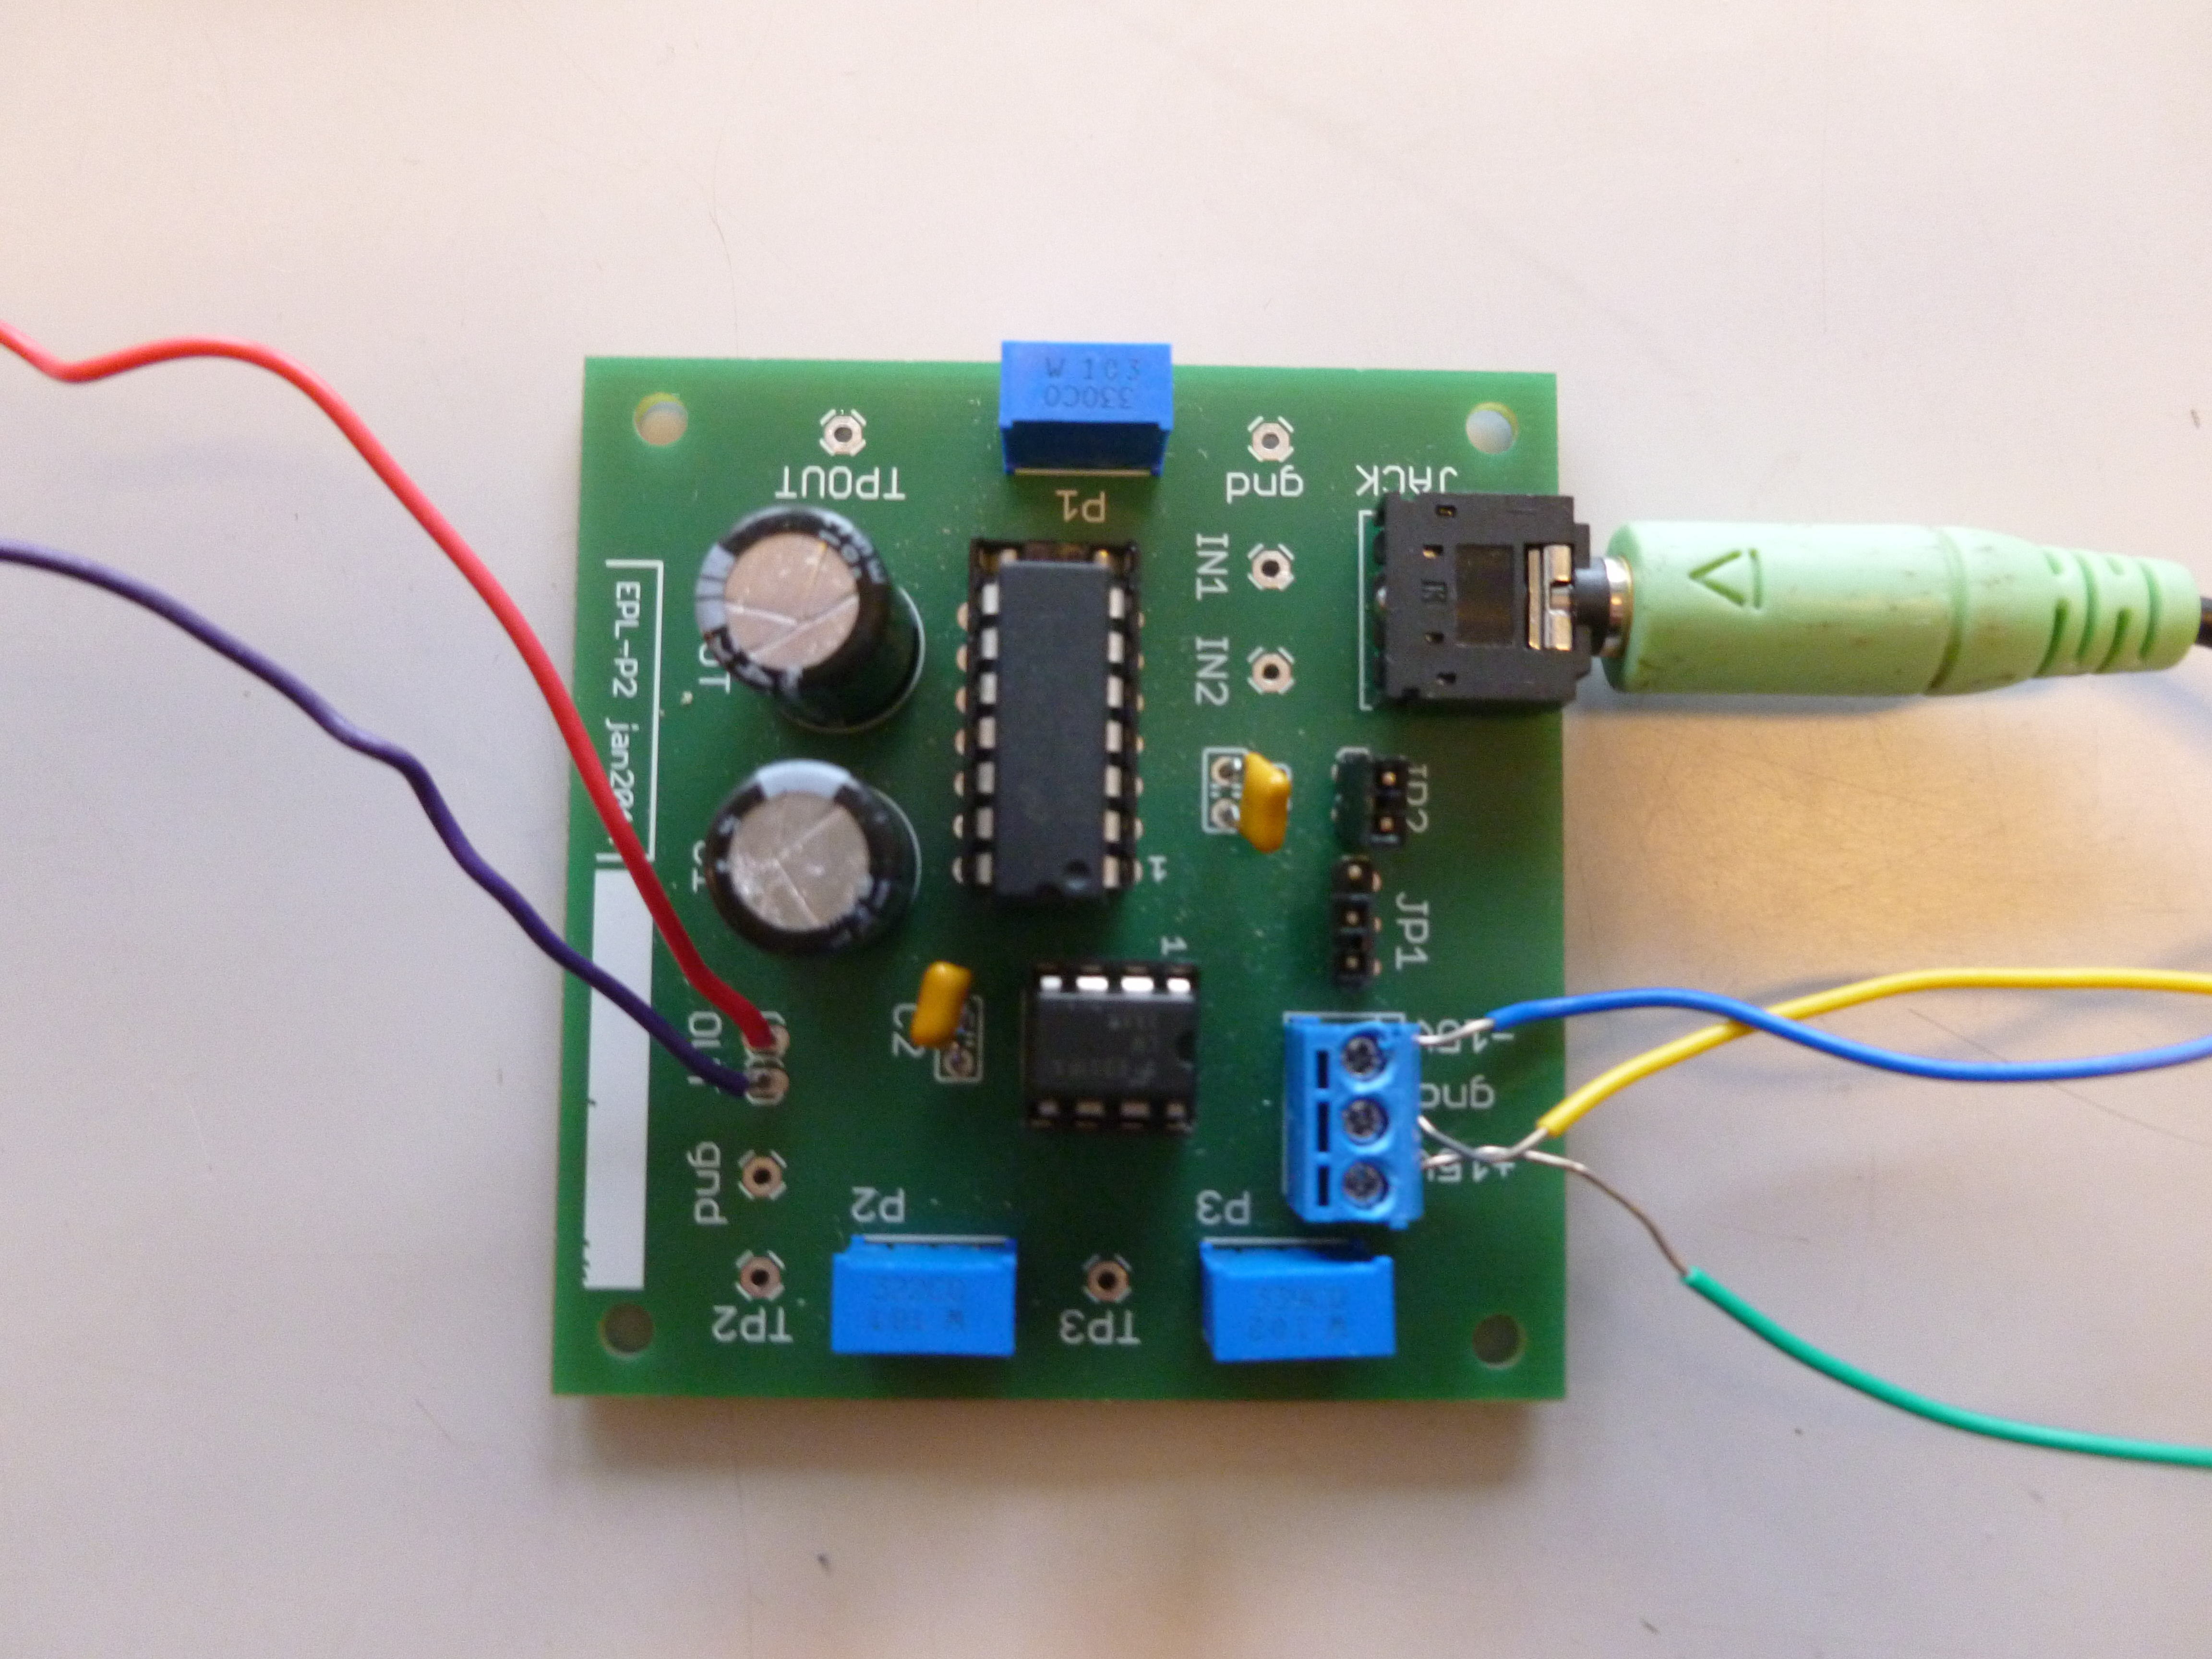
\includegraphics[scale=0.05]{P1010039.jpg}
    \caption{Schéma de la plaquette}
    \label{plaquette}
\end{figure}


%La méthode des mesures est expliquée

Nous avons fait des mesures de voltage en fonction de différentes fréquences pour les filtres RC: ce qui nous a permis
de trouver les fréquences de coupures. Pour mesurer les différentes valeurs reprises ci dessous, nous avons procédé de la
façon suivante: nous avons branché deux générateurs à la plaquette: Une source positive branchée à la borne $+15$ de la plaquette. 
Une source négative branchée à la borne $-15$ de la plaquette.  La terre est quant à elle branchée au dernier point 
disponible de la plaquette: gnd (pour ground).  De plus, la terre est branchée aux sources positives et négatives 
restantes.  Quand nous mesurons la tension aux différents points nous nous servons d'un oscilloscope.  Avec la sonde,
nous touchons le circuit où nous voulons savoir la valeur de la tension.  Sur l'écran, on voit apparaitre le 
signal, en réglant l'appareil sur le bon ordre de grandeur, nous pouvons mesurer assez précisement la tension en 
tel ou tel point.  En annexe, on peut voir des photos des phases de tests. 
  Nous avons fait ces tests avec les filtres
passe haut et passe bas.  Cela correspond au bloc 1 et 2.

\begin{figure}[ht!]
    \centering
    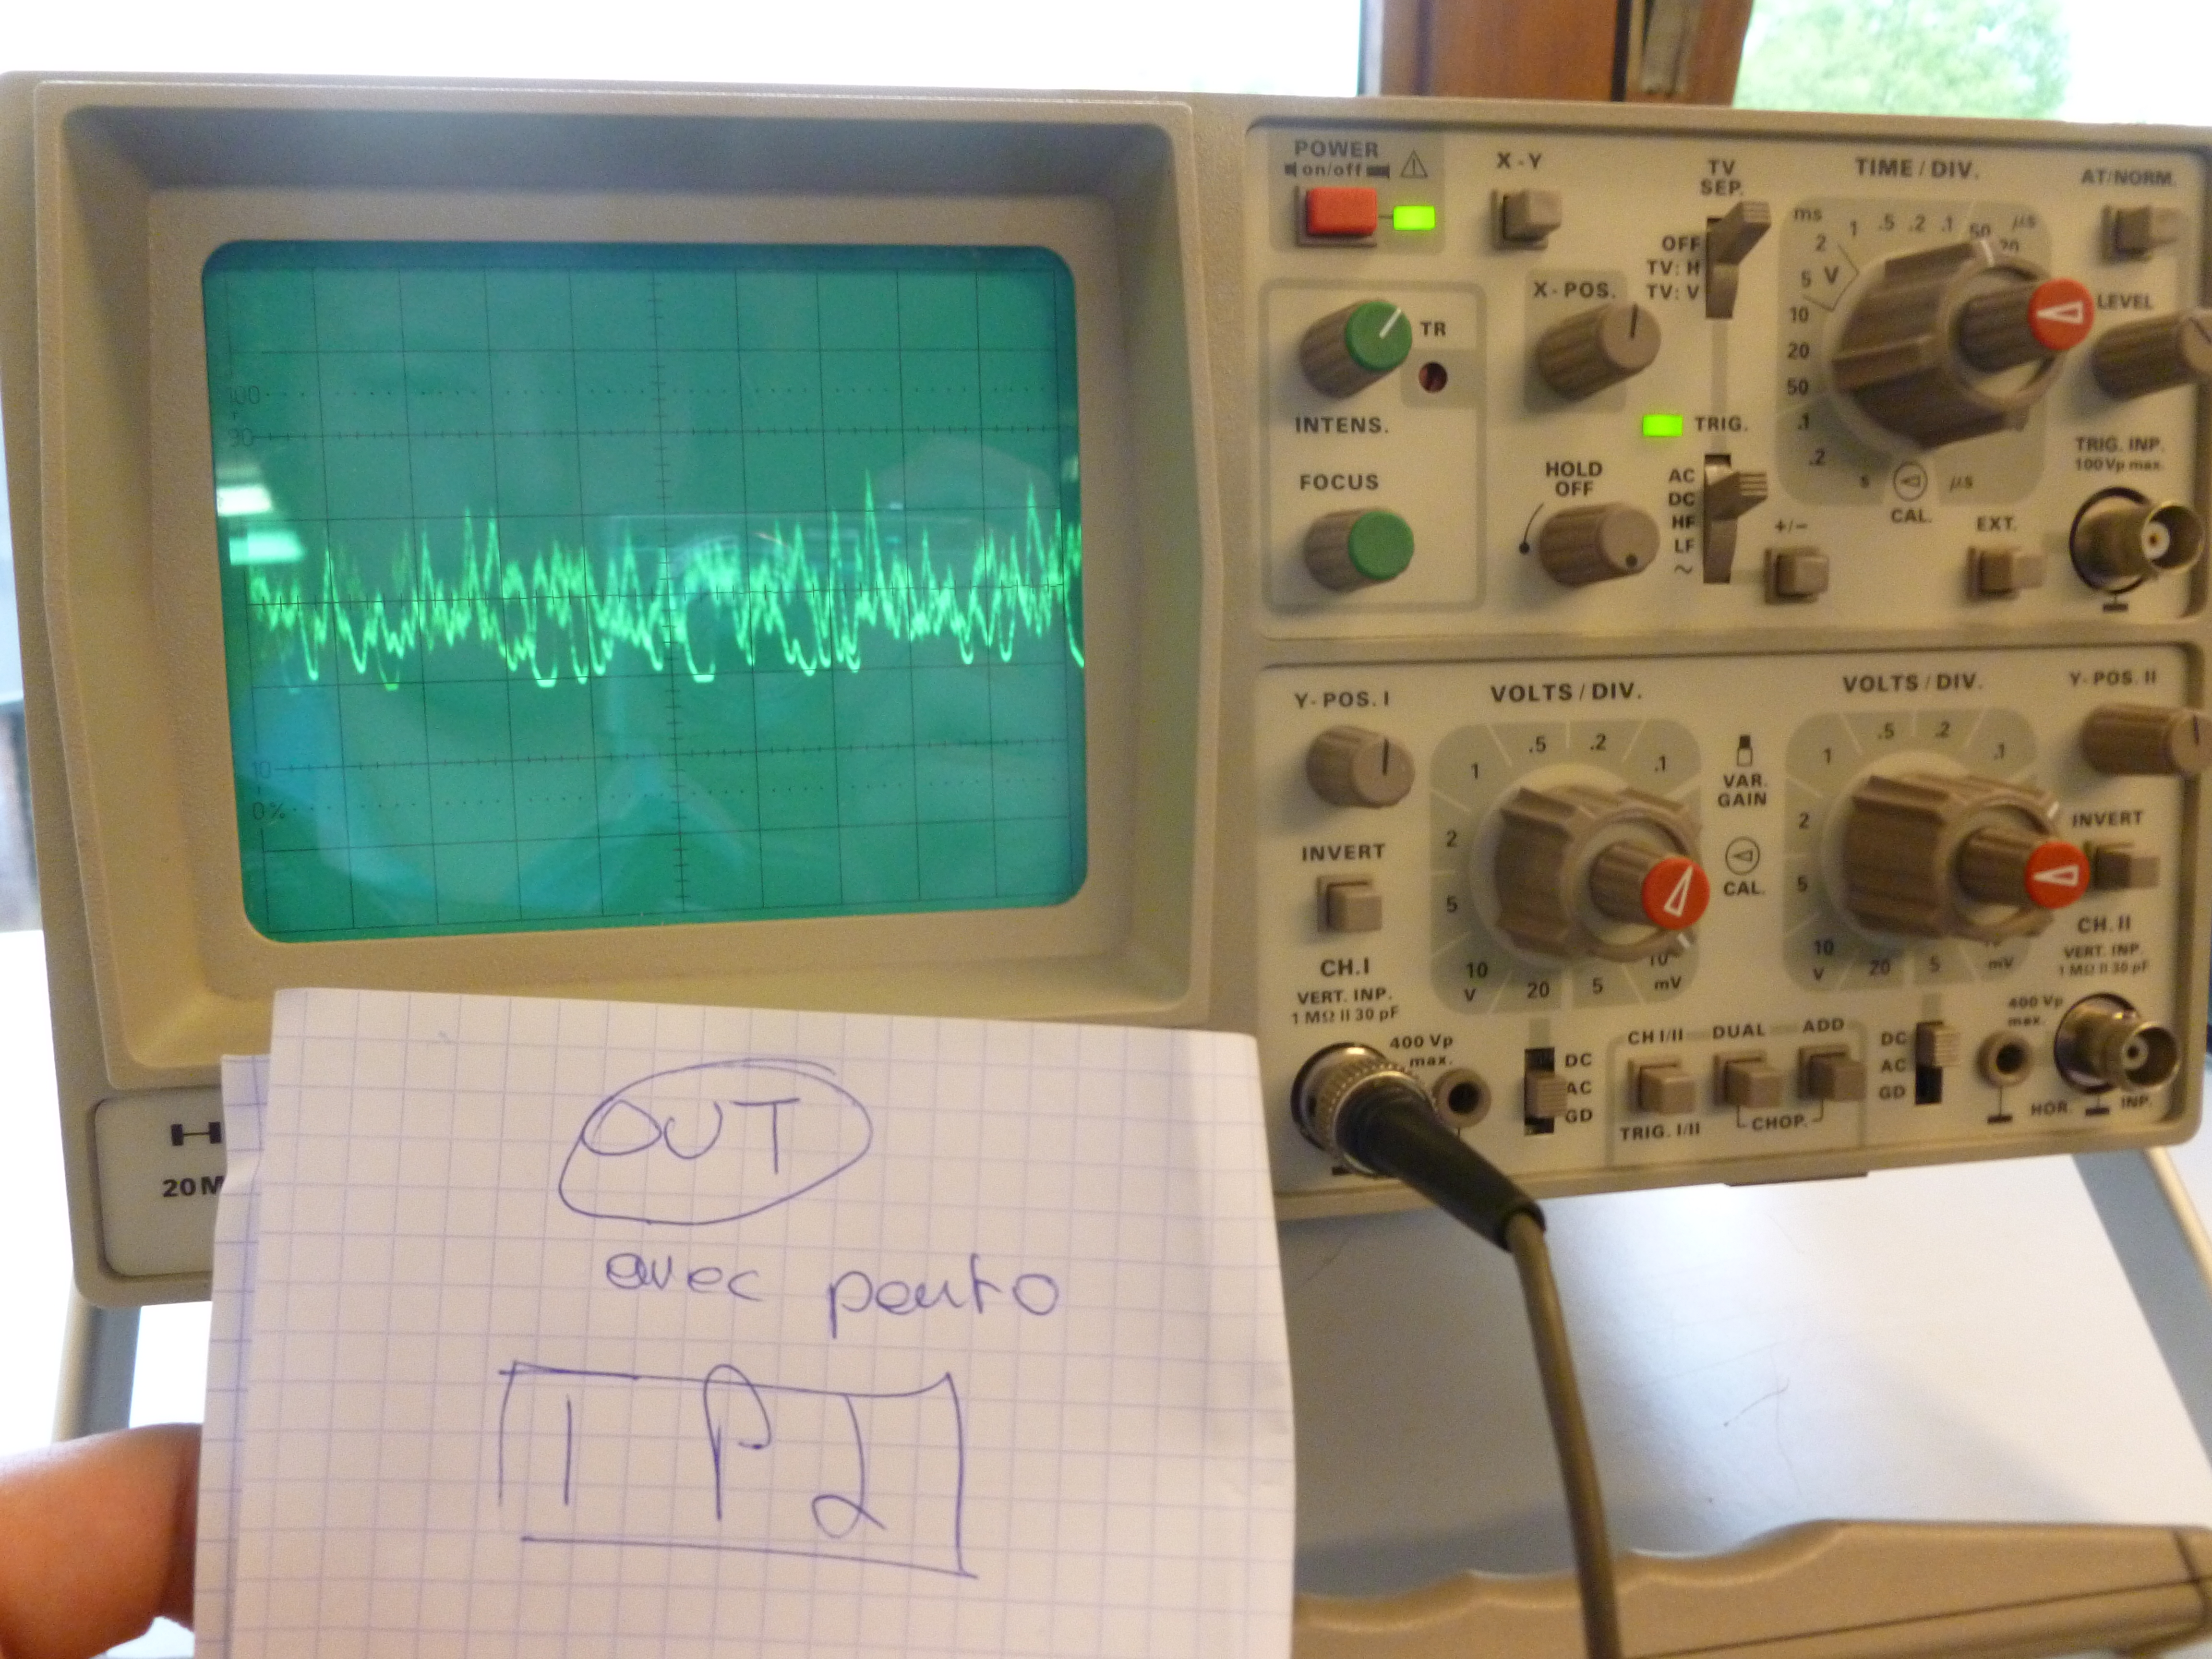
\includegraphics[scale=0.05]{P1010038.jpg}
    \caption{Oscilloscope}
    \label{Oscilloscope pour TP2}
\end{figure}


Pour la bobine fixe, nous voulions savoir quel était le champs produit par les bobines, pour cela nous avons fait passer
du courant dans les bobines en reliant un générateur avec les fils de la bobine et nous avons mis le capteur du teslamètre 
dans l'entrefer.  Après, nous lisions la valeur du champs sur l'écran de l'appareil.
Quand nous mesurions la resistance des bobines, nous isolions la bobine que nous voulions tester, on la branche au multimètre
et on regarde la valeur, nous veillons à chaque fois à bien avoir le bon ordre de grandeur. Cela renvoit au bloc 3.

Enfin, nous avons fait des tests sur la sortie de la plaquette, en testant avec l'oscilloscope.  Nous regardions l'écran de
l'appareil pour voir si une fréquence possible sortait de la plaquette.  Cela correspond au bloc 4.

\emph{Précautions}
\begin{enumerate}
\item Lors de chaque test, il est nécessaire de laisser les objets immobiles pour éviter des erreurs dû à leur mobilité.
\item Eviter que les fils ne touchent la plaque verte, qui est la masse.


%Des tests paramétriques sont effectués

Nous avons décidé de faire nos essais avec une tension de plus et moins 15 V car l'ampli-op nécéssite une tension
de maximum plus et moins 16.5 V, nous prenons un peu moins pour avoir une marge de sécurité.
Il est clair que si nous changeons cette valeure et que nous mettons plus de tension, le son sera plus amplifié vu que 
la plaquette aura une plus grande source de tension.  


En faisant augmenter les aigus, nous voyons que le signal est plus condensé et vice versa.

Quand nous mettons plus de courant dans la bobine fixe, un plus grand champs magnétique est créé, mais trop l'augmenter
ferait fondre le fil.

\begin{figure}[ht!]
    \centering
    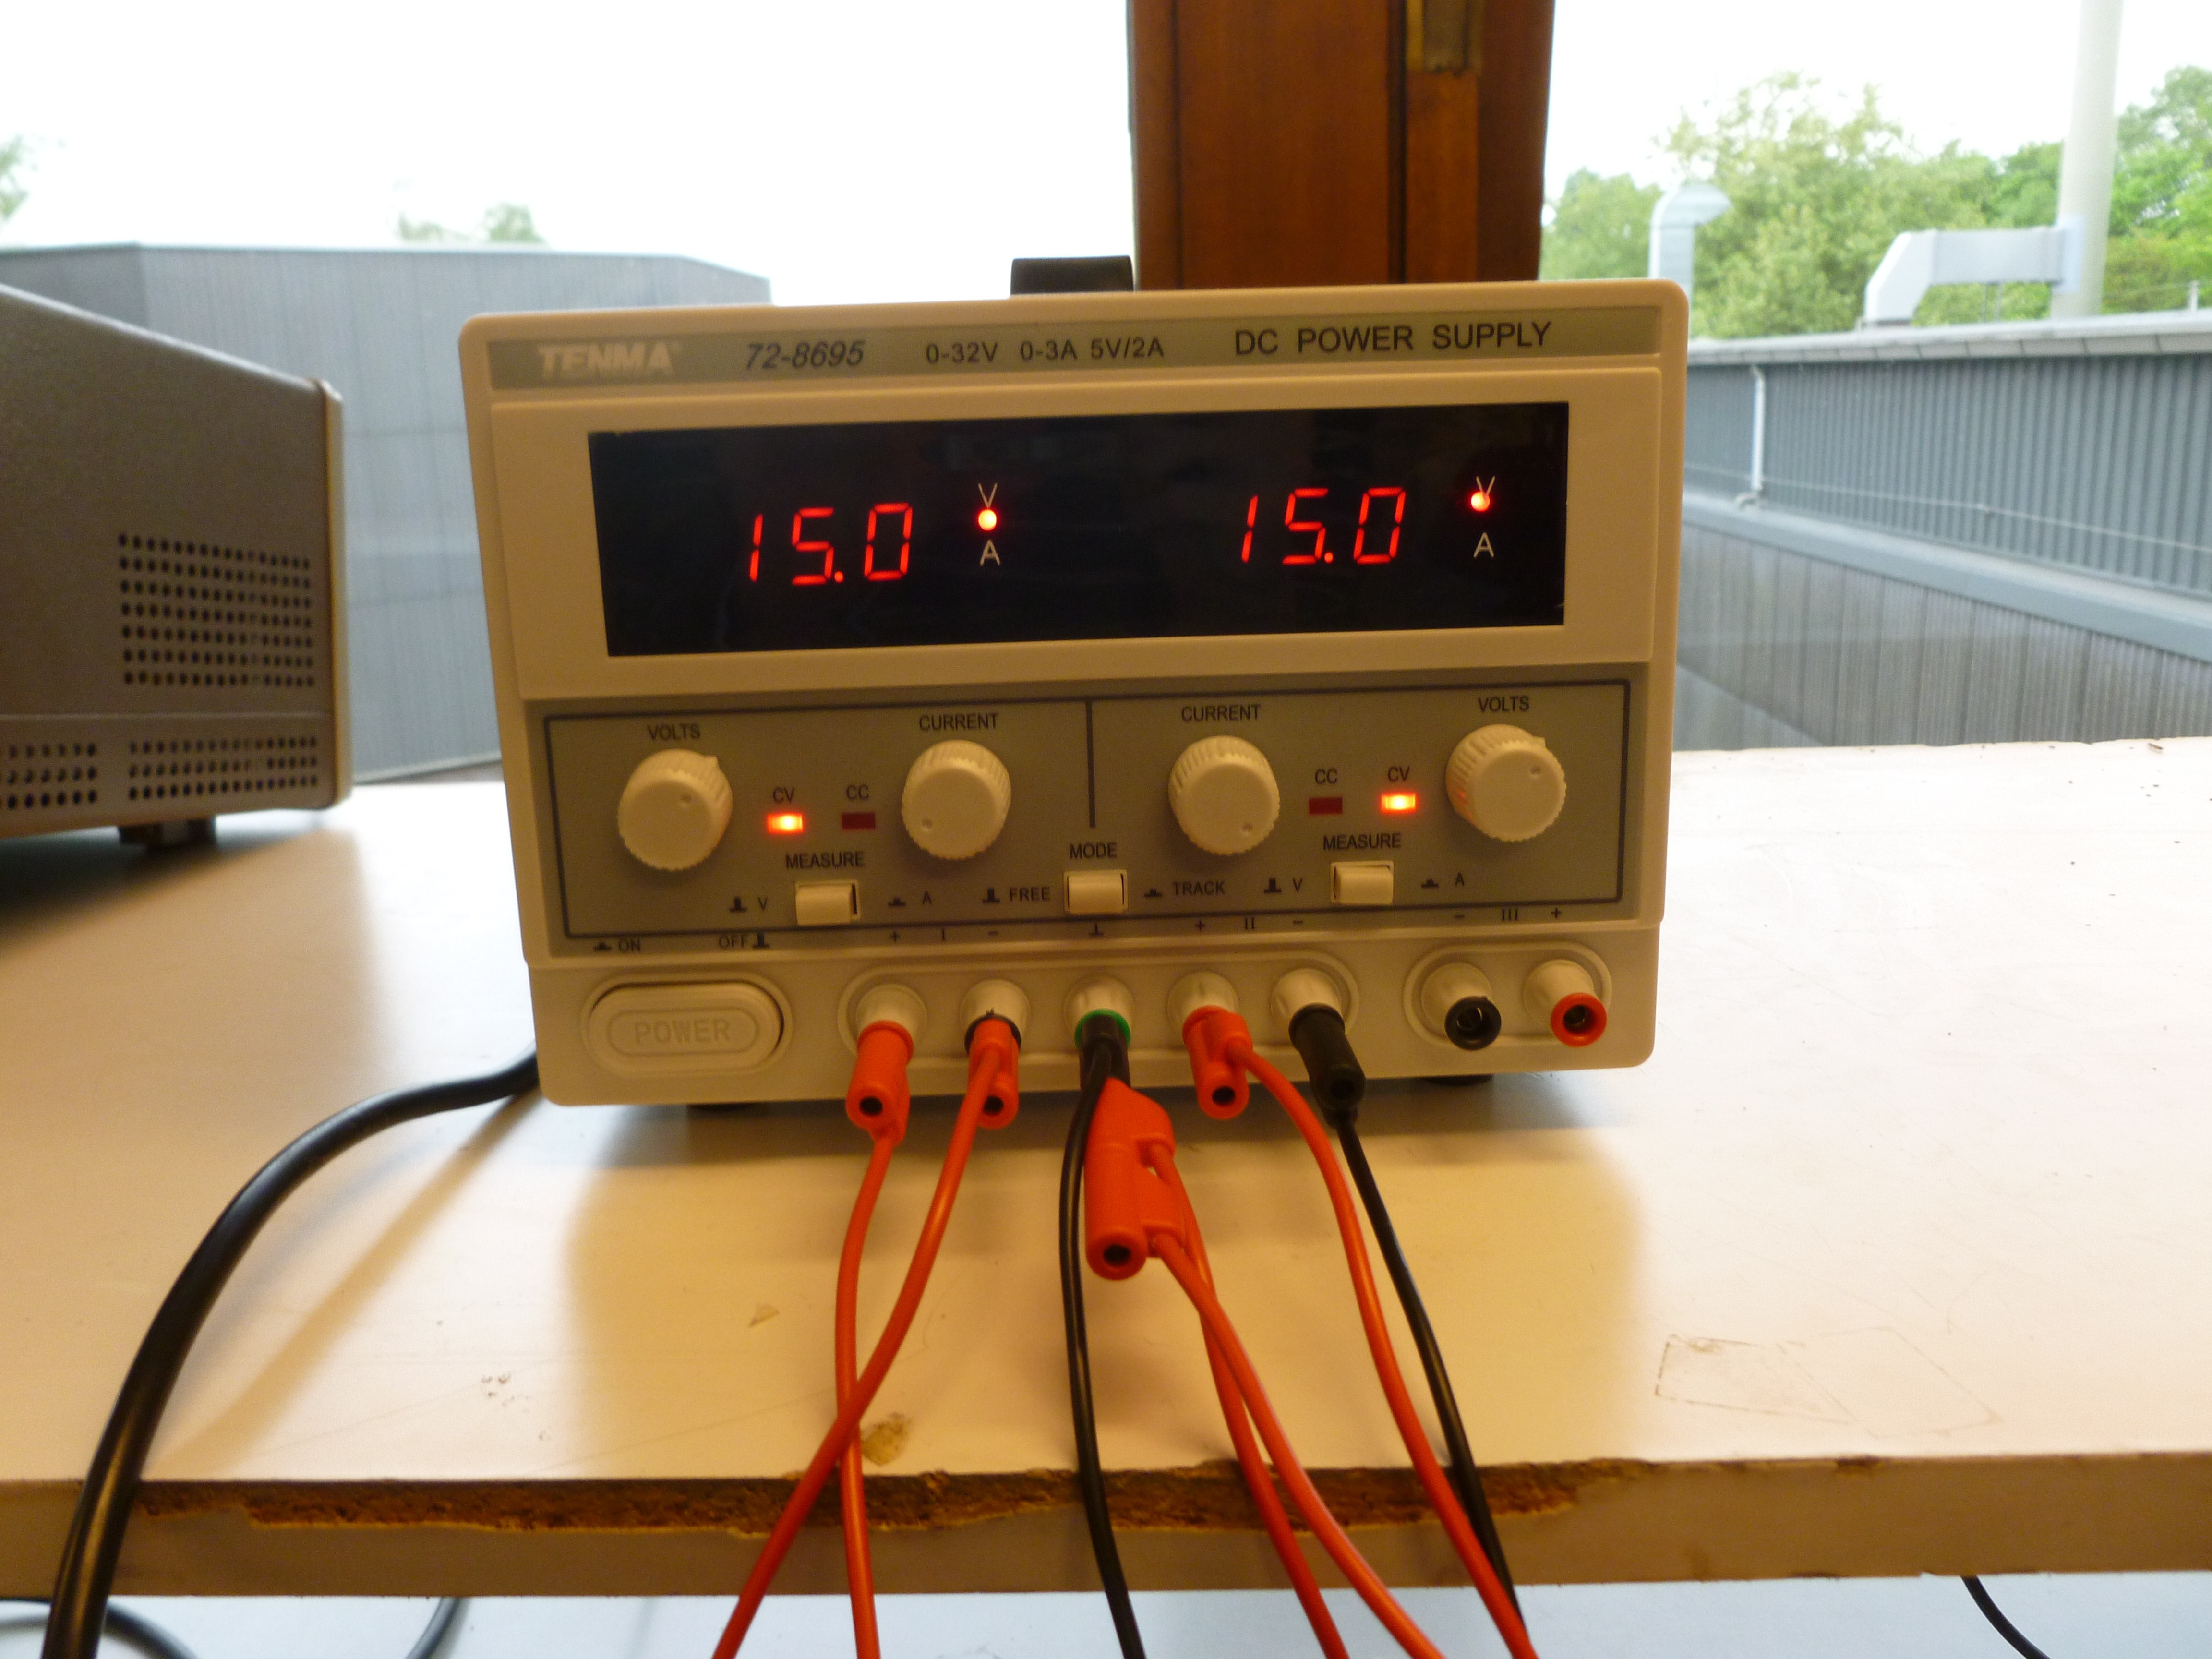
\includegraphics[scale=0.05]{P1010031.jpg}
    \caption{Générateurs}
    \label{Branchements des générateurs}
\end{figure}

%Mesures
Pour le filtre passe-bas:
\begin{center}
\begin{tabular}{|c|c|c|}
\hline
$V_c[V]$ & $f[Hz]$ & $\log{f}$ \\
\hline
1.7 & 16000 & 4.204 \\
\hline
1.55 & 18000 & 4.255 \\
\hline
1.45 & 20000 & 4.301 \\
\hline
\end{tabular}
\end{center}

Pour le filtre passe-haut

\begin{center}
	\begin{tabular}{|c|c|c|}
		\hline
		$V_c[V]$ & $f[Hz]$ & $\log{f}$ \\
		\hline
		127 & 0.4 & 2.1\\
		\hline
		191 & 0.5 & 2.3\\
		\hline
		356 & 0.6 & 2.6 \\
		\hline
	\end{tabular}
\end{center}

\begin{center}
	\begin{tabular}{|c|c|c|}
		\hline
		$Resistance bobine fixe[\ohms]$ & $Champ magn.[T]$ & $Amperage[A]$ \\
		\hline
		2.38 & 0.08 & 0.1667\\
		\hline
	\end{tabular}
\end{center}

\begin{document}

\begin{center}
\begin{tabular}{|c|c|c|c|c|}
\hline
$Prise Jack [mV]$ & $IN_1 [mV]$ & $OUT_{avec  pentotiomètre} [V]$ & $OUT_{sans pentotiomètre} [V]$ & $TP_2 [mV]$ \\
		\hline
		 37.5 & 100.0 & 0.22 & 3.0 & 11.0 \\
		\hline
	\end{tabular}
\end{center}





% Just here to fix rapport_prejury.tex
\end{document}


\chapter{Discussion et conclusion}

\documentclass{article}

\usepackage[utf8]{inputenc}
\usepackage[T1]{fontenc}      
\usepackage[francais]{babel}
\usepackage{graphicx}
\usepackage{circuitikz}
\usepackage[squaren, Gray]{SIunits}
\usepackage{sistyle}
\usepackage[autolanguage]{numprint}
\usepackage{pgfplots}
\usepackage{amsmath,amssymb,array}
\usepackage{url} 

% New command pour la modélisation mécanique, tri à effectuer
\newcommand\fv[1]{{\bf #1}} % free vector
\newcommand\fvd[1]{\dot{\bf #1}} % free vector derivated
\newcommand\fvdd[1]{\ddot{\bf #1}} % free vector derivated
\newcommand\fvr[1]{\mathring{\bf #1}} % free vector relatively derivated
\newcommand\fvrr[1]{\overset{\circ\circ}{\bf #1}} % free vector relatively derivated
\newcommand\uv[1]{{\bf\hat{ #1}}} % unit vector
\newcommand\ui{{\bf\hat{I}}} % unit vector I
\newcommand\uj{{\bf\hat{J}}} % unit vector J
\newcommand\uk{{\bf\hat{K}}} % unit vector K
\newcommand\wrt[2]{\ensuremath{\tensor*[_{ #1}]{ #2}{}}} % With Respect To
\newcommand\wtr[3]{\ensuremath{\tensor*[_{ #1}]{ #2}{^{ #3}}}} % With Two Respect
\newcommand\omegaf{{\bm \omega}}
\newcommand\omegafr{\mathring{\bm \omega}}
\newcommand\omegafd{\dot{\bm \omega}}
\newcommand\omegaft{\tilde{\bm \omega}}
\newcommand\omegaftr{\mathring{\tilde{\bm \omega}}}
\newcommand\omegat{\tilde{\omega}}
\newcommand\omegatd{\tilde{\dot{\omega}}}
\newcommand\ine{{\bf I}}
\newcommand\st{{\bf L}}
\newcommand\pst{{\bf M}}
\newcommand\lm{{\bf N}}
\newcommand\am{{\bf H}}
\newcommand\amd{\dot{\am}}
\newcommand\fo{{\bf F}}
\newcommand\po{\mathcal{P}}
\newcommand\xg{\ensuremath{\fv{R}}}
\newcommand\xgd{\ensuremath{\fvd{R}}}
\newcommand\xgdd{\ensuremath{\fvdd{R}}}
\newcommand\dvec[1]{\dot{\vec{ #1}}}
\newcommand\ddvec[1]{\ddot{\vec{ #1}}}
\newcommand\qp{\dot{q}}
\newcommand\dqp{\Delta \dot{q}}

\begin{document}


% Théorie et pratique
En théorie, un son devrait sortir du haut-parleur.  En pratique, il y a bien une fréquence
à la sortie de la plaquette mais le haut-parleur demeure aphone. Il y a donc manifestement 
un mauvais raccordement bobine fixe-bobine mobile.

% Mesure et modélisation
Les mesures réalisées sont moins précises que la simulation, mais nous obtenons tout de même 
des valeurs plus petite que celle attendues.  Par exemple, nous obtenons un champ magnétique
expérimental plus faible que calculé.  Cela est tout à fait normal vu que nous avons émis des
des hypothèses simplificatrices qui ne respectent pas tout à fait la réalité. Nous avions 
imposé la conservation du flux dans nos calculs, par exemple. Il est évident que des pertes de flux 
ont été subies, et tout le flux n'étais pas concentré dans l'entrefer, malgré que nous l'ayons minimisé.

% Système complet
Les points forts de notre système sont les suivants: la membrane, le caisson, et l'entrefer. La membrane a 
été réalisée avec du tissus et du papier, et ainsi éviter les pliages difficiles, mais tout de même garder 
une certaine rigidité.  Le caisson est également un fierté, étant donné qu'il a été pensé pour obtenir le
meilleur rapport qualité-prix. Enfin, nous avons pensé à réduire l'entrefer, pour maximiser le champ magnétique.
Le principal point faible de l'appareil est qu'il n'y a pas de son sortant du haut-parleur.

% Gestion du travail de groupe
Nous avons assez bien géré le groupe, l'ambiance dans le groupe était excellente.  Le travail était assez bien réparti
même si ce n'était pas possible que tout le monde ait la même charge de travail.  Grâce à des outils comme GitHub, Dropbox et 
\Latex, la communication pour la rédaction du rapport à été grandement facilitée.

% Just here to fix rapport_prejury.tex
\end{document}
\clearpage

\documentclass{article}

\usepackage[utf8]{inputenc}
\usepackage[T1]{fontenc}      
\usepackage[francais]{babel}
\usepackage{graphicx}
\usepackage{circuitikz}
\usepackage[squaren, Gray]{SIunits}
\usepackage{sistyle}
\usepackage[autolanguage]{numprint}
\usepackage{pgfplots}
\usepackage{amsmath,amssymb,array}
\usepackage{url} 

% New command pour la modélisation mécanique, tri à effectuer
\newcommand\fv[1]{{\bf #1}} % free vector
\newcommand\fvd[1]{\dot{\bf #1}} % free vector derivated
\newcommand\fvdd[1]{\ddot{\bf #1}} % free vector derivated
\newcommand\fvr[1]{\mathring{\bf #1}} % free vector relatively derivated
\newcommand\fvrr[1]{\overset{\circ\circ}{\bf #1}} % free vector relatively derivated
\newcommand\uv[1]{{\bf\hat{ #1}}} % unit vector
\newcommand\ui{{\bf\hat{I}}} % unit vector I
\newcommand\uj{{\bf\hat{J}}} % unit vector J
\newcommand\uk{{\bf\hat{K}}} % unit vector K
\newcommand\wrt[2]{\ensuremath{\tensor*[_{ #1}]{ #2}{}}} % With Respect To
\newcommand\wtr[3]{\ensuremath{\tensor*[_{ #1}]{ #2}{^{ #3}}}} % With Two Respect
\newcommand\omegaf{{\bm \omega}}
\newcommand\omegafr{\mathring{\bm \omega}}
\newcommand\omegafd{\dot{\bm \omega}}
\newcommand\omegaft{\tilde{\bm \omega}}
\newcommand\omegaftr{\mathring{\tilde{\bm \omega}}}
\newcommand\omegat{\tilde{\omega}}
\newcommand\omegatd{\tilde{\dot{\omega}}}
\newcommand\ine{{\bf I}}
\newcommand\st{{\bf L}}
\newcommand\pst{{\bf M}}
\newcommand\lm{{\bf N}}
\newcommand\am{{\bf H}}
\newcommand\amd{\dot{\am}}
\newcommand\fo{{\bf F}}
\newcommand\po{\mathcal{P}}
\newcommand\xg{\ensuremath{\fv{R}}}
\newcommand\xgd{\ensuremath{\fvd{R}}}
\newcommand\xgdd{\ensuremath{\fvdd{R}}}
\newcommand\dvec[1]{\dot{\vec{ #1}}}
\newcommand\ddvec[1]{\ddot{\vec{ #1}}}
\newcommand\qp{\dot{q}}
\newcommand\dqp{\Delta \dot{q}}

\begin{document}


\section{Conclusion}

Nous voici finalement arrivés au terme de notre projet. Il y a douze semaines de cela, aucun 
d'entre nous ne connaissait le fonctionnement d'un haut-parleur. Aucun d'entre nous ne savait vraiment utiliser 
le matériel d'un laboratoire. Aucun de nous ne maîtrisait entièrement ne fût-ce qu'une parcelle de ce que nous 
avons appris. Aujourd'hui, nous pouvons nous targuer d'avoir énormément progressé; que ce soit d'un point de
vue scientifique, mathématique, ou organisationnel. Il est temps maintenant de prendre du recul, et jeter un 
regard critique sur ce que nous avons accompli.

% bilan aux niveaux scientifiques et techniques
\paragraph{Formation scientifique et technique}
Ce projet nous a permis de mettre en pratique de nombreuses notions abordées aux cours de mathématiques et
de physique, que ce soit au premier ou au second quadrimestre. 
Au niveau scientifique, nous avons abordé différents concepts physiques clefs comme la loi d'\textsc{Ampère},
la force de \textsc{Laplace}, la loi de \textsc{Hooke}, mais également tout ce qui concerne la 
magnétostatique dans le vide et la matière, les matériaux magnétiques, les filtres passe-haut et passe-bas,...
De plus, nous avons été amenés à nous renseigner sur la distorsion harmonique et la contre-réaction, pour 
finalement rédiger un résumé de ce que nous avions appris.
Au niveau technique, nous avons compris et assimilé le fonctionnement théorique d’un haut-parleur, nous avons
étudié le circuit imprimé et ses composants, nous avons utilisé les fiches de spécifications de certains 
éléments et matériaux pour en tirer ce qui nous intéressait, nous avons étudié la mécanique de la membrane
ainsi que bien d'autres aspects encore.
À chaque question que nous nous sommes posée, nous nous sommes efforcés d'apporter des réponses techniques 
de qualité.

% bilan au niveau de la gestion: forces et faiblesses  + décisions importantes
\paragraph{Organisation et travail de groupe}
Étant donné que nous avions déjà participé à un projet au premier quadrimestre, nous avons pu en exploiter 
notre expérience.  Pour la plupart des membres du groupe, le projet était plus structuré dans notre groupe
actuel que dans les anciens. Nous avons effectivement essayé de faire un juste partage des tâches, et chaque
membre a pu apporter sa contribution. Un autre point à relever est le fait que le groupe est resté soudé 
pendant toute la durée du projet. Tout le monde était présent aux séances sauf en cas de force majeure. 
Cependant, nous n'avons pas assez privilégié les réunions réelles, étant donné que nous travaillions de notre
côté pour seulement mettre en commun par la suite. Par conséquent, le même travail était parfois réalisé
plusieurs fois. Un meilleur rendement aurait fait avancer le projet plus rapidement et plus intelligemment.
Cependant, toutes les grandes décisions telles que le fait de se focaliser sur un seul haut-parleur lorsque 
nous avons commencé à manquer de temps, ont été prises en groupe.

% outils pour le travail
Un dernier point important concernant le travail de groupe est l'utilisation d'outils pour la mise en commun.
Le fait que nous utilisions les mêmes outils a facilité l’échange de documents et d’informations. 
Par exemple, nous avons fait l’effort d’apprendre \LaTeX pour écrire notre rapport; nous avons également créé
une Dropbox ainsi qu’un compte GitHub où tous les documents étaient modifiables à tout moment du jour et de 
la nuit. Lorsqu'un changement était effectué, tous les membres du groupe en étaient avertis. 
Notons tout de même que nous n'avons pas négligé la réunion physique puisqu'elle reste 
le meilleur moyen de communiquer. 
% planning utilisé pr les échéances + commentaire
Grâce au planning réalisé lors du pré-jury, nous avons su avancer dans le projet de manière organisée et 
claire. Il nous a bien servi pour acquérir une vision structurée du projet, des échéances
et des délivrables. Malgré quelques écarts, nous nous sommes assez bien tenus au plan. Des problèmes répétitifs 
au niveau du circuit imprimé ont cependant retardé notre réalisation, et c'est ainsi que notre haut-parleur 
n'est pas tout à fait fonctionnel au final. À part cela, le cahier des charges a été respecté dans son ensemble.

% cohérence entre cdc et ccls
En conclusion, même si le haut-parleur ne fonctionnait pas comme nous le souhaitions, les concepts 
mathématiques et physiques ont été tout à fait assimilés. Notre groupe est resté solidaire durant tout 
le quadrimestre; prenant le temps de s'assurer de la compréhension de chacun. Ce projet nous aura donc été
grandement profitable, et c'est avec une grande fierté que nous y apportons le point final.

% Just here to fix rapport_prejury.tex
\end{document}

\clearpage

% Bibliographie
\bibliography{sources}
\bibliographystyle{plain}
\nocite{*}

\chapter{Annexes}

\documentclass{article}

\usepackage[utf8]{inputenc}
\usepackage[T1]{fontenc}
\usepackage[francais]{babel}
\usepackage{amsmath,amssymb,array}
 
\begin{document}
 
\section{Approximation de la fréquence de coupure}

\subsection{Pour le filtre passe-bas}

\subsubsection{Equation de la droite horizontale} % A refaire avec la méthode d'approximation
Nous savons que la droite horizontale a une valeur initiale de 2.5 V et donc \[y=2.5\]

\subsubsection{Equation de la droite diagonale}

Nous savons que l'équation de la droite est de type $y=a*x+b$
\\
Mais pour cette situation-ci, nous allons utiliser une base logarithmique pour la pente.  En effet, les différentes fréquences utilisées sont tellement éloignées les unes des autres que le graphique serait gigantesque et la pente diagonale serait en fait une courbe.  Ce qui donne: $y=a*\log{x}+b$

Voici 3 résultats mesurés en laboratoire.

\bigbreak
\\
\begin{tabular}{|c|c|c|}
\hline
V_c & f & log{ f} \\
\hline
1.7 & 16000 & 4.204\\
\hline
1.55 & 18000 & 4.255\\
\hline
1.45 & 20000 & 4.301 \\
\hline
\end{tabular}

\bigbreak
Des maintenant les fréquences sont exprimées en base logarithmique et nous obtenons la matrice suivante :
\bigbreak

$$
\begin{pmatrix}  
 4.204 & 1\\
 4.255 & 1 \\
 4.301 & 1 
\end{pmatrix}
\begin{pmatrix}  
a\\
b
\end{pmatrix}
=
\begin{pmatrix}  
1.7\\
1.55\\
1.45
\end{pmatrix}
$$

\bigbreak

Ce qui nous donne les vecteurs suivants:

\[e_1=( \frac{1}{\sqrt[]{3}} \frac{1}{\sqrt[]{3}} \frac{1}{\sqrt[]{3}})\]

\\ et

\\
\[e_2=( -0.68, 0.03, 0.73)\]

\bigbreak
Ce qui nous donne une projection de 
$$
\begin{pmatrix}  
1.6\\
1.5\\
1.4
\end{pmatrix}$$
$$

\bigbreak
Nous en déduisons la valeur des coefficients a et b:  
\[ a =-1.96 \]
\[ b= 9.84 \]

$$\fbox{y= -1.96 \timeslog{x} +9.84}$$

\bigbreak
Pour trouver la fréquence d'intersection entre les deux droites $$y=2.5$$ et $$y= -1.96 \times log{x} +9.84$$ nous égalisons les y et nous trouvons $$\fbox{x=5557.7 Hz$$} 

\\
Cela nous semble correct car en théorie nous devons arriver à une valeur f tel que $$f=\frac{1}{2\times \pi\times R\times C}$$
avec $R=7.5+50=57.5 ohms$ et $C=470\times 10^{-9} F$  Notre valeur théorique de la fréquence est donc $$f=5889.2 Hz$$


\subsection{Pour le filtre passe-haut}

\subsubection{Equation de la droite horizontale}

Nous savons que la droite a une valeur initiale de 0.75 V et donc \[y=0.75\]

\subsubsection{Equation de la droite diagonale}

Nous savons que l'équation de la droite est de type $y=a*x+b$
\\
Mais pour cette situation-ci, nous allons utiliser une base logarithmique pour la pente.  En effet, les différentes fréquences utilisées sont tellement éloignées les unes des autres que le graphique serait gigantesque et la pente diagonale serait en fait une courbe.  Ce qui donne: $y=a*\log{x}+b$


Voici 3 résultats mesurés en laboratoire.
\bigbreak
\\
\begin{tabular}{|c|c|c|}
\hline
V_c & f & log{ f} \\
\hline
127 & 0.4 & 2.1\\
\hline
191 & 0.5 & 2.3\\
\hline
356 & 0.6 & 2.6 \\
\hline
\end{tabular}

\bigbreak
Des maintenant les fréquences sont exprimées en base logarithmique et nous obtenons la matrice suivante:
\bigbreak
$$
\begin{pmatrix}  
 2.1 & 1\\
 2.3 & 1 \\
 2.6 & 1 
\end{pmatrix}
\begin{pmatrix}  
a\\
b
\end{pmatrix}
=
\begin{pmatrix}  
0.4\\
0.5\\
0.6
\end{pmatrix}
$$
\bigbreak

Ce qui nous donne les vecteurs suivants:

\[e_1=( \frac{1}{\sqrt[]{3}} \frac{1}{\sqrt[]{3}} \frac{1}{\sqrt[]{3}})\]

\\ et

\\
\[e_2=( -0.6, 0, 0.8)\]

\bigbreak
Ce qui nous donne une projection de 
$$
\begin{pmatrix}  
0.36\\
0.5\\
0.69
\end{pmatrix}$$
$$

\bigbreak
Nous en déduisons la valeur des coefficients a et b:  
\[ a =0.7 \]
\[ b= -1.11 \]

$$\fbox{y= -1.96 \timeslog{x} +9.84}$$

\bigbreak
Pour trouver la fréquence d'intersection entre les deux droites $$y=0.75$$ et $$y= 0.7 \times log{x} -1.11$$ nous égalisons les y et nous trouvons $$\fbox{x=439.4 Hz$$} 

\end{document}

\clearpage

\documentclass{article}

\usepackage[utf8]{inputenc}
\usepackage[T1]{fontenc}      
\usepackage[francais]{babel}
\usepackage{graphicx}
\usepackage{circuitikz}
\usepackage[squaren, Gray]{SIunits}
\usepackage{sistyle}
\usepackage[autolanguage]{numprint}
\usepackage{pgfplots}
\usepackage{amsmath,amssymb,array}
\usepackage{url} 

% New command pour la modélisation mécanique, tri à effectuer
\newcommand\fv[1]{{\bf #1}} % free vector
\newcommand\fvd[1]{\dot{\bf #1}} % free vector derivated
\newcommand\fvdd[1]{\ddot{\bf #1}} % free vector derivated
\newcommand\fvr[1]{\mathring{\bf #1}} % free vector relatively derivated
\newcommand\fvrr[1]{\overset{\circ\circ}{\bf #1}} % free vector relatively derivated
\newcommand\uv[1]{{\bf\hat{ #1}}} % unit vector
\newcommand\ui{{\bf\hat{I}}} % unit vector I
\newcommand\uj{{\bf\hat{J}}} % unit vector J
\newcommand\uk{{\bf\hat{K}}} % unit vector K
\newcommand\wrt[2]{\ensuremath{\tensor*[_{ #1}]{ #2}{}}} % With Respect To
\newcommand\wtr[3]{\ensuremath{\tensor*[_{ #1}]{ #2}{^{ #3}}}} % With Two Respect
\newcommand\omegaf{{\bm \omega}}
\newcommand\omegafr{\mathring{\bm \omega}}
\newcommand\omegafd{\dot{\bm \omega}}
\newcommand\omegaft{\tilde{\bm \omega}}
\newcommand\omegaftr{\mathring{\tilde{\bm \omega}}}
\newcommand\omegat{\tilde{\omega}}
\newcommand\omegatd{\tilde{\dot{\omega}}}
\newcommand\ine{{\bf I}}
\newcommand\st{{\bf L}}
\newcommand\pst{{\bf M}}
\newcommand\lm{{\bf N}}
\newcommand\am{{\bf H}}
\newcommand\amd{\dot{\am}}
\newcommand\fo{{\bf F}}
\newcommand\po{\mathcal{P}}
\newcommand\xg{\ensuremath{\fv{R}}}
\newcommand\xgd{\ensuremath{\fvd{R}}}
\newcommand\xgdd{\ensuremath{\fvdd{R}}}
\newcommand\dvec[1]{\dot{\vec{ #1}}}
\newcommand\ddvec[1]{\ddot{\vec{ #1}}}
\newcommand\qp{\dot{q}}
\newcommand\dqp{\Delta \dot{q}}

\begin{document}


\section{Projet specifications}

\begin{table*} [h]

\begin{tabular}{|l|c|l|}

\hline
&&\\
\textbf{Group} & & \hfill \textbf{Date}  March 7th 2014\\
11.53 && \hfill \textbf{Version} 2.1\\

\hline
\multicolumn{3}{|p{15cm}|}{\textbf{Context} \newline
Our goal during this project is to realize, qualify, and measure an amplification system. This device should allow us to hear smartphone signals from two loudspeakers. The volume and the intensity of the bass and treble sounds should be adjustable.}  \\


\hline
\textbf{Date} & \textbf{Origine} & \textbf{Content}\\
\hline
&&\\
&&\textbf{Principal functions}\\
&&\\
16/02/14 & Costumer & 1. Emit a sound \\
16/02/14 & Costumer & 2. Amplify a sound \\
16/02/14 & Costumer & 3. Variation of bass and treble \\
&&\\
\hline
&&\\
& & \textbf{Criteria and level of the main functions} \\
&&\\
16/02/14 & Group & 1.1. Sound between ... and... Hz \\
16/02/14 & Costumer & 2.1. Power of 2.5 W \\
&&\\
\hline
&&\\
& & \textbf{Constraints} \\
&&\\
16/02/14 & Costumer &   Jackplug of 3.5 mm in diameter\\
16/02/14 & Laboratory &  Input voltage of 30V \\
07/03/14 & Costumer&  Paper membrane \\
&&\\
\hline
&&\\
& & \textbf{Terms} \\
&&\\
07/03/14 & Group & Type of paper : 200 g/m$^{2}$ \\
07/03/14 & Group & Cost estimation : ...\\

&&\\
\hline
\end{tabular}

\end{table*}

\end{document}

\clearpage

\documentclass{article}

\usepackage[utf8]{inputenc}
\usepackage[T1]{fontenc}      
\usepackage[francais]{babel}
\usepackage{graphicx}
\usepackage{circuitikz}
\usepackage[squaren, Gray]{SIunits}
\usepackage{sistyle}
\usepackage[autolanguage]{numprint}
\usepackage{pgfplots}
\usepackage{amsmath,amssymb,array}
\usepackage{url} 

% New command pour la modélisation mécanique, tri à effectuer
\newcommand\fv[1]{{\bf #1}} % free vector
\newcommand\fvd[1]{\dot{\bf #1}} % free vector derivated
\newcommand\fvdd[1]{\ddot{\bf #1}} % free vector derivated
\newcommand\fvr[1]{\mathring{\bf #1}} % free vector relatively derivated
\newcommand\fvrr[1]{\overset{\circ\circ}{\bf #1}} % free vector relatively derivated
\newcommand\uv[1]{{\bf\hat{ #1}}} % unit vector
\newcommand\ui{{\bf\hat{I}}} % unit vector I
\newcommand\uj{{\bf\hat{J}}} % unit vector J
\newcommand\uk{{\bf\hat{K}}} % unit vector K
\newcommand\wrt[2]{\ensuremath{\tensor*[_{ #1}]{ #2}{}}} % With Respect To
\newcommand\wtr[3]{\ensuremath{\tensor*[_{ #1}]{ #2}{^{ #3}}}} % With Two Respect
\newcommand\omegaf{{\bm \omega}}
\newcommand\omegafr{\mathring{\bm \omega}}
\newcommand\omegafd{\dot{\bm \omega}}
\newcommand\omegaft{\tilde{\bm \omega}}
\newcommand\omegaftr{\mathring{\tilde{\bm \omega}}}
\newcommand\omegat{\tilde{\omega}}
\newcommand\omegatd{\tilde{\dot{\omega}}}
\newcommand\ine{{\bf I}}
\newcommand\st{{\bf L}}
\newcommand\pst{{\bf M}}
\newcommand\lm{{\bf N}}
\newcommand\am{{\bf H}}
\newcommand\amd{\dot{\am}}
\newcommand\fo{{\bf F}}
\newcommand\po{\mathcal{P}}
\newcommand\xg{\ensuremath{\fv{R}}}
\newcommand\xgd{\ensuremath{\fvd{R}}}
\newcommand\xgdd{\ensuremath{\fvdd{R}}}
\newcommand\dvec[1]{\dot{\vec{ #1}}}
\newcommand\ddvec[1]{\ddot{\vec{ #1}}}
\newcommand\qp{\dot{q}}
\newcommand\dqp{\Delta \dot{q}}

\begin{document}


% A revoir
\section{Planning}

Au début du quadrimestre, il nous a été demandé de concevoir, réaliser et quantifier un système de haut-parleur. Notre travail
a été répartie en trois partie : les séances tutorées, les laboratoires et le travail autonome. Dés le début de notre projet,
 plusieurs tâches nous ont été demandé : réaliser une recherche biblographique, concevoir un cahier des charges,
dimensionner notre haut-parleur, ect. 


\subsection{Avant le pré-jury}
Après 6 semaines de travail sur notre projet du deuxième quadrimestre, voici où en était l'état d'avancement 
de notre projet:

Nous avons décidé après un brain-strorming en groupe de centrer notre recherche bibliographique sur la distorsion harmonique 
et la boucle de contre-réaction présente dans notre circuit. Nous nous sommes documentés durant plusieurs semaines pour avoir
une recherche bibliographique la plus complète.

Une des première tâche importante de notre projet est de réaliser un cahier des charges. Nous avons posé les fonctions principales
et les contraintes de notre projet lors de la première semaine. Durant l'avancement de notre projet, nous l'avons complété
 afin d'améliorer au mieux les fonctions et contraintes ainsi que poser les dimensions de notre haut-parleur.

Dés la première semaine, nous nous sommes familiarisé avec les appareils en laboratoire pour ensuite travailler sur les
deux filtres passe-haut et passe-bas de notre circuit. Nous avons mesurer les tensions de sortie de ces blocs en fonction
de différentes capacités et résistances. Nous avons ensuite commencé à souder une partie des composantes sur nos plaquettes.

En parallèle, nous avons réalisé l'analyse mathématique et physique du filtre passe-bas ainsi que le dimensionnement de la bobine
pour l'électro-aimant. Une fois les dimensions définies, nous avons pu commencer à bobiner les différentes bobines.

Une esquisse de la membrane pour le haut-parleur a été proposé tout en sachant que quelques modifications restait à faire.

\subsection{Après le pré-jury}

Dés la semaine 9, nous nous sommes plus concentré sur la fabrication même du haut-parleur : nous avons commencé par la
membrane en papier et tissus que nous avons testé par la suite. Nous avons aussi réaliser les caisons en bois contenant notre
circuit et l'électro-aimant.

Nous nous étions fixé pour la semaine 11 d'avoir fini de souder les deux plaquettes pour les tests de validation. Malheureusement,
ayant eu quelques problème avec notre première plaquette, nous avons préféré rester concentrer sur celle-ci et ne pas terminer
la seconde. 

Après les tests de validations, nous avons remis en commun tout le travail effectué les semaines précédentes pour s'atteler
à la rédaction de notre rapport.
Dans les semaines à venir, nous prévoyons de préparer notre défense oral (préparation des slides, répartitions des temps 
de paroles, ect.).

Globalement nous avons su respecter en temps les différentes de notre projet en répartissant la tâche de travail de manière
équilibré sur les différentes semaines. Néanmoins, les dernières semaines ont été plus chargé avec la construction du haut parleur 
et de la rédaction de notre rapport.

\textbf{Ancienne version}

\subsection{Ce qui restait à faire}

Pour les semaines d'après pré-jury nous avions orgagnisé notre temps de la manière suivante:

\begin{enumerate}
	\item{S9}: Finaliser la conception de la membrane et la tester.
	\item{S10}: Réaliser le caisson dans lequel on mettra notre circuit ainsi que la membrane.
	\item{S11}: Souder entièrement la deuxième plaque pour faire notre deuxième haut-parleur (si le premier haut-parleur fonctionne).
	\item{S11}: Réaliser le deuxième haut-parleur en suivant les plans du premier.
	\item{S12}: Centraliser tous les travaux (bien mettre tout en ordre) et rédiger le rapport final.
	\item{S13}: Slides pour le jury-final
	\item{S14}: Préparation de la défense orale et achever les slides.
\end{enumerate}

Nous pouvons dire que nous nous sommes assez bien tenu au planning durant toute la 2ème partie du quadrimestre. 
Mis à part que le deuxième haut-parleur n'a pas été entièrement réalisé ( nous préférions nous concentrer d'abord sur 
le premier), les étapes ont été réalisées en temps et en heure.  La charge de travail était assez bien équilibrée sur 
les différentes semaines même si nous avons dû travailler plus dur dans les dernières semaines pour construire le haut-parleur
et rédiger le rapport.
% Just here to fix rapport_prejury.tex
\end{document}

\clearpage

\documentclass{article}

\usepackage[utf8]{inputenc}
\usepackage[T1]{fontenc}      
\usepackage[francais]{babel}
\usepackage{graphicx}
\usepackage{circuitikz}
\usepackage[squaren, Gray]{SIunits}
\usepackage{sistyle}
\usepackage[autolanguage]{numprint}
\usepackage{pgfplots}
\usepackage{amsmath,amssymb,array}
\usepackage{url} 

% New command pour la modélisation mécanique, tri à effectuer
\newcommand\fv[1]{{\bf #1}} % free vector
\newcommand\fvd[1]{\dot{\bf #1}} % free vector derivated
\newcommand\fvdd[1]{\ddot{\bf #1}} % free vector derivated
\newcommand\fvr[1]{\mathring{\bf #1}} % free vector relatively derivated
\newcommand\fvrr[1]{\overset{\circ\circ}{\bf #1}} % free vector relatively derivated
\newcommand\uv[1]{{\bf\hat{ #1}}} % unit vector
\newcommand\ui{{\bf\hat{I}}} % unit vector I
\newcommand\uj{{\bf\hat{J}}} % unit vector J
\newcommand\uk{{\bf\hat{K}}} % unit vector K
\newcommand\wrt[2]{\ensuremath{\tensor*[_{ #1}]{ #2}{}}} % With Respect To
\newcommand\wtr[3]{\ensuremath{\tensor*[_{ #1}]{ #2}{^{ #3}}}} % With Two Respect
\newcommand\omegaf{{\bm \omega}}
\newcommand\omegafr{\mathring{\bm \omega}}
\newcommand\omegafd{\dot{\bm \omega}}
\newcommand\omegaft{\tilde{\bm \omega}}
\newcommand\omegaftr{\mathring{\tilde{\bm \omega}}}
\newcommand\omegat{\tilde{\omega}}
\newcommand\omegatd{\tilde{\dot{\omega}}}
\newcommand\ine{{\bf I}}
\newcommand\st{{\bf L}}
\newcommand\pst{{\bf M}}
\newcommand\lm{{\bf N}}
\newcommand\am{{\bf H}}
\newcommand\amd{\dot{\am}}
\newcommand\fo{{\bf F}}
\newcommand\po{\mathcal{P}}
\newcommand\xg{\ensuremath{\fv{R}}}
\newcommand\xgd{\ensuremath{\fvd{R}}}
\newcommand\xgdd{\ensuremath{\fvdd{R}}}
\newcommand\dvec[1]{\dot{\vec{ #1}}}
\newcommand\ddvec[1]{\ddot{\vec{ #1}}}
\newcommand\qp{\dot{q}}
\newcommand\dqp{\Delta \dot{q}}

\begin{document}


\section{Méthode de recherche}

\subsection{La contre-réaction ou réaction négative}
Comme suggeré lors de la séance d'information sur la recherche bibliographique,
nous avons appliqué la méthode de l'entonnoir. Comme les boucles de contre-réaction 
sont directement liées aux amplificateurs, nous avons commencé nos recherches avec 
les termes plutôt généraux : \textit{amplificateurs} et \textit{amplifiers}. Nous 
nous avons ensuite associé à ces mots clés les termes plus précis : \textit{contre-réaction}
et \textit{negative feedback}.

Les différents ouvrages et documents que nous avons utilisés sont listés dans la bibliographie.

\subsection{La distorsion harmonique}

\paragraph{Choix du thème}
Le choix du thème n'a pas été chose aisée. Nous avons commencé par établir un brainstorming afin de réunir 
le plus d'idées possibles. Cependant, les thèmes proposés nous semblaient trop généraux que pour faire un vrai 
travail en profondeur tout en restant concis. Quelqu'un a finalement proposé la distorsion harmonique ; un 
terme visible sur les emballages de haut-parleurs. Nous avions également repéré ce terme dans la datasheet 
de l'amplificateur audio reçu pour le projet: une valeur de \numprint{0.2\%} était renseignée pour le THD 
(taux de distorsion harmonique). Curieux d'en apprendre plus sur ce terme presque méconnu, 
nous avons décidé de débuter notre travail de recherche là-dessus.

\paragraph{Recherche documentaire}
Etant donné que nous ne connaissions vraiment que très peu sur ce sujet et que nous 
devions le comprendre en profondeur, nous avons commencé par le terme général de "distorsion".
Une première recherche sur internet a permis de fixer les idées à propos de ce terme, et nous 
avons ensuite pu établir une liste de mot-clefs pour entamer réellement la recherche sur la 
distorsion harmonique. Nous avons appliqué la "technique de l'entonnoir", et nous avons finalement 
réuni assez d'informations que pour écrire ce rapport. Notons tout de même que c'est indiscutablement
en anglais que nous avons 
trouvé le plus d'informations. Nous avons gardé une trace de toutes les sources que nous avons 
consultées, et cela a rendu l'écriture de la bibliographie nettement plus facile.

% Just here to fix rapport_prejury.tex
\end{document}

\clearpage

\documentclass{article}

\usepackage[utf8]{inputenc}
\usepackage[T1]{fontenc}      
\usepackage[francais]{babel}
\usepackage{graphicx}
\usepackage{circuitikz}
\usepackage[squaren, Gray]{SIunits}
\usepackage{sistyle}
\usepackage[autolanguage]{numprint}
\usepackage{pgfplots}
\usepackage{amsmath,amssymb,array}
\usepackage{url} 

% New command pour la modélisation mécanique, tri à effectuer
\newcommand\fv[1]{{\bf #1}} % free vector
\newcommand\fvd[1]{\dot{\bf #1}} % free vector derivated
\newcommand\fvdd[1]{\ddot{\bf #1}} % free vector derivated
\newcommand\fvr[1]{\mathring{\bf #1}} % free vector relatively derivated
\newcommand\fvrr[1]{\overset{\circ\circ}{\bf #1}} % free vector relatively derivated
\newcommand\uv[1]{{\bf\hat{ #1}}} % unit vector
\newcommand\ui{{\bf\hat{I}}} % unit vector I
\newcommand\uj{{\bf\hat{J}}} % unit vector J
\newcommand\uk{{\bf\hat{K}}} % unit vector K
\newcommand\wrt[2]{\ensuremath{\tensor*[_{ #1}]{ #2}{}}} % With Respect To
\newcommand\wtr[3]{\ensuremath{\tensor*[_{ #1}]{ #2}{^{ #3}}}} % With Two Respect
\newcommand\omegaf{{\bm \omega}}
\newcommand\omegafr{\mathring{\bm \omega}}
\newcommand\omegafd{\dot{\bm \omega}}
\newcommand\omegaft{\tilde{\bm \omega}}
\newcommand\omegaftr{\mathring{\tilde{\bm \omega}}}
\newcommand\omegat{\tilde{\omega}}
\newcommand\omegatd{\tilde{\dot{\omega}}}
\newcommand\ine{{\bf I}}
\newcommand\st{{\bf L}}
\newcommand\pst{{\bf M}}
\newcommand\lm{{\bf N}}
\newcommand\am{{\bf H}}
\newcommand\amd{\dot{\am}}
\newcommand\fo{{\bf F}}
\newcommand\po{\mathcal{P}}
\newcommand\xg{\ensuremath{\fv{R}}}
\newcommand\xgd{\ensuremath{\fvd{R}}}
\newcommand\xgdd{\ensuremath{\fvdd{R}}}
\newcommand\dvec[1]{\dot{\vec{ #1}}}
\newcommand\ddvec[1]{\ddot{\vec{ #1}}}
\newcommand\qp{\dot{q}}
\newcommand\dqp{\Delta \dot{q}}

\begin{document}


\section{Analyse séquentielle du circuit}
Dans cette section, nous allons décrire le fonctionnement du circuit
de notre haut-parleur de la manière la plus précise et la plus complète
possible. 

Cette section est découpée en quatre sections, une pour chaque bloc 
principal du circuit. Chaque bloc est associé à un rôle bien précis du
haut-parleur.

\paragraph{Remarque}
Dans cette section, la figure associé à chaque composant sera constituée
d'un schéma de ce composant à gauche et d'une photo de ce composant à droite.

\subsection{La connexion avec la prise Jack}

\begin{figure}[!hbt]
	\centering
	\includegraphics[scale=0.6]{jack-female.png}
	\includegraphics[scale=0.24]{jack-female-r.jpg}
	\caption{Premier bloc du circuit :
					la prise Jack femelle. (Source : datasheet du composant sur Farnell.com)}
	\label{jack-female}
\end{figure}

Ce premier bloc (Figure \ref{jack-female}), chargé de faire la connexion 
entre la source (smartphone, iPod, etc) et le reste du circuit, est constitué de la prise Jack femelle. 
Pour bien comprendre son fonctionnement, regardons d'abord à quoi ressemble la prise Jack
mâle avec laquelle elle sera couplée (Figure \ref{jack-plug}).

\begin{figure}[!hbt]
	\centering
	\includegraphics[scale=0.1]{jack-plug.png}
	\caption{Prise Jack mâle \unit{3.5}{\milli\meter}, contact en 3 points. (Source : Wikipédia)}
	\label{jack-plug}
\end{figure}

Cette prise Jack mâle sert à transporter un signal stéréophonique, qui sépare le 
canal gauche et le canal droit. Le canal gauche correspond à la pointe de la prise 
(L sur la figure), le canal droit correspond à l'anneau de la prise (R sur la figure). 
Le manchon de la prise correspond quant à lui à la masse.

Sur le schéma de la prise Jack femelle (Figure \ref{jack-female}), nous pouvons alors
voir que le signal du canal droit sortira du point \numprint{6}, tandis que le signal du 
canal gauche sortira du point \numprint{7}. La terre est quant à elle reliée au point
\numprint{3}. Sur le dessin de la plaquette (Figure \ref{dessin-pcb}), on remarque alors
que c'est le signal du canal droit qui sera traité par la plaquette, celui-ci se dirigeant vers
le point \textit{IN1}. Le canal gauche, dirigé quant à lui vers le point \textit{IN2} pourrait
être récupéré et dirigé vers une deuxième plaquette afin que nos deux haut-parleurs soient en stéréo.

\begin{figure}[!hbt]
	\centering
	\includegraphics[scale=0.5]{dessin-pcb.png}
	\caption{Dessin de la face avant du circuit imprimé. (Source : Composants pour le projet P2, iCampus)}
	\label{dessin-pcb}
\end{figure}

\subsection{Le réglage du volume}
Le fonctionnement de ce bloc est relativement simple à comprendre, il est constitué d'un potentiomètre 
(P1 sur la Figure \ref{dessin-pcb}), c'est-à-dire d'une résistance variable.
Selon la valeur de la résistance, par la loi d'Ohm, l'amplitude du signal
sera plus ou moins réduite et donc le volume sera plus ou moins grand.

\begin{figure}[!hbt]
	\centering
	\includegraphics[scale=1.1]{pot.png}
	\includegraphics[scale=0.30]{pot-r.jpg}
	\caption{Potentiomètre. (Soure : datasheet du composant sur Farnell.com)}
	\label{bloc2}
\end{figure}

Nous disposions de 3 potentiomètres pour réaliser notre haut-parleur, possédant
tous une résistance maximale différente :

\begin{center}
	\begin{tabular}{l|r}
	3386W-1-101-LF & \unit{100}{\ohm} \\
	3386W-1-102-LF & \unit{1000}{\ohm} \\
	3386W-1-103-LF & \unit{10000}{\ohm} 
	\end{tabular}
\end{center}

% A verifier
Afin de permettre une plus grande variation du volume, nous avons décidé d'utiliser
le potentiomètre avec la plus grande résistance maximale en \textit{P1}.

\subsection{Le réglage des graves et des aigus}
Ce bloc-ci est sans aucun doute le plus compliqué à comprendre. Il est constitué d'un 
filtre passe-haut (réglage des aigus) et d'un filtre passe-bas (réglage des graves).
Le filtre passe-haut est celui qui suit le premier amplificateur (\textit{LM358N-A}),
le passe-bas est celui qui suit le deuxième amplificateur (\textit{LM358N-B}). 
La combinaison des deux filtres forme un filtre passe-bande, représenté sur la
Figure \ref{filtre}. 

\begin{figure}[!hbt]
	\centering
	\includegraphics[scale=0.6]{filtre-passe-bande.png}
	\caption{Schéma électrique du filtre passe-bande de notre haut-parleur.
	(Source : Composants pour le projet P2, iCampus)}
	\label{filtre}
\end{figure}

Ce bloc est un petit peu plus compliqué à situer sur la Figure
\ref{dessin-pcb} car les deux amplificateurs sont situés dans le Dual ampli-op (LM358N) 
représenté à la Figure \ref{dual-ampli-op}. 

\begin{figure}[!hbt]
	\centering
	\includegraphics[scale=0.6]{dual-opamp.png}
	\includegraphics[scale=0.45]{dual-opamp-r.jpg}
	\caption{Le dual op-amp. (Source : datasheet du composant sur Farnell.com)}
	\label{dual-ampli-op}
\end{figure}

Ce dual ampli-op est alimenté en $\unit{\pm15}{\volt}$ par l'intermédiaire
d'un bornier.

Un autre point intéressant à relever sur le schéma du filtre est la présence d'une boucle 
reliant la sortie à la borne négative de chaque amplificateur. Ces boucles sont appelées
"boucles de contre-réaction".  Le gain normal d'un amplificateur est de l'ordre de $10^{6}$. 
Grâce aux boucles de contre-réaction, on peut contrôler le gain d'un amplificateur. 
Dans notre cas, le gain de l'amplificateur est ramené à $1$. 
Les deux amplificateurs sont ce qu'on appelle des \textit{suiveurs de tensions}. 
Leur rôle est de permettre le règlage des graves et des aigus de manière indépendante.
Sans ces amplificateurs suiveurs, faire varier le potentiomètre \textit{P2} influencerait 
non seulement le filtre passe-haut, mais influencerait aussi le filtre passe-bas 
(car les potentiomètres \textit{P2} et \textit{P3} sont en série).

Chaque filtre (passe-haut et passe-bas) est composé d'un potentiomètre et d'une capacité céramique
(Figure \ref{capac-r}) de \unit{470}{\nano\farad}.

\begin{figure}[!htb]
	\centering
	\includegraphics[scale=0.4]{capac-r.jpg}
	\caption{Capacité céramique utilisée dans les filtres. (Source : datasheet du composant sur Farnell.com)}
	\label{capac-r}
\end{figure}

% VERIFÉ
Afin d'assurer à notre haut-parleur la plus grande bande passante, nous avons utilisé le potentiomètre
dont la résistance maximale est de \unit{1000}{\ohm}) pour le filtre passe-haut et
l'autre (dont la résistance maximale est de \unit{100}{\ohm}) pour le filtre passe-bas. En effet, soient
$f_1$ et $f_2$ les fréquences de coupures respectives des filtres passe-haut et passe-bas, la norme de la 
bande passante est donnée par :

$$f_2 - f_1$$

Pour avoir la plus grande bande passante, il faut donc :

$$f_1 < f_2 \Rightarrow \frac{1}{2\pi R_1C} < \frac{1}{2\pi R_2C} \Rightarrow R_2 < R_1$$

Le choix inverse aurait pu aboutir à une bande passante nulle.

Concernant le câble reliant les points 1 du Jumper 1 (\textit{JP1}) et du Jumper 2 (\textit{JP2}), 
il s'agit en quelque sorte d'un câble de "sécurité" que l'on peut connecter afin que le signal 
ne passe pas par les filtres passe-haut et passe-bas. 
Cela pourrait nous être utile pour tester notre haut-parleur dans l'hypothèse où un des filtres 
ne fonctionnerait pas.

Enfin, nous pouvons aussi remarquer une boucle qui relie le point 1 du potentiomètre 3 (\textit{P3})
au reste du circuit. Cette boucle a simplement pour but d'éviter de laisser un câble "`dans le vide"',
et donc d'éviter les signaux parasites.

\subsection{L'amplificateur de puissance}

\begin{figure}[!htb]
	\centering
	\includegraphics[scale=0.48]{ampli-audio.png}
	\includegraphics[scale=0.35]{ampli-audio-r.jpg}
	\caption{L'amplificateur de puissance. (Source : datasheet du composant sur Farnell.com)}
	\label{ampli-audio}
\end{figure}

Cette partie contient l'amplificateur de puissance (aussi appelé amplificateur audio). 
Cet amplificateur a pour but d'amplifier un signal électrique audio pour
permettre le fonctionnement d'un haut-parleur ou d'une enceinte acoustique.

Le nom amplificateur de puissance peut induire en erreur. En effet, comme tout amplificateur,
l'amplificateur de puissance agit sur la tension mais son impédance de sortie étant très faible,
il peut délivrer une grande puissance (ce qui lui vaut son nom).

Dans notre cas, l'amplificateur a un gain en tension de \numprint{50} et une puissance de $\unit
{2.5}{\watt}$.
% A vérifier pour la puissance, la liste des composants laisse penser qu'il s'agit plutôt de 2W
% sur la date sheet il est mis 2.5 W

Le premier condensateur \textit{C1} (Figure \ref{dessin-pcb}) sert à stabiliser la tension 
d'alimentation de l'amplificateur audio, qui est de \unit{15}{\volt}. 

Le deuxième condensateur (\textit{COUT}) (Figure \ref{dessin-pcb}) permet de ne laisser passer 
que les signaux alternatifs. Il bloque tous les courants continus parasites.

Ces deux condensateurs polarisés ont une capacitance de \unit{470}{\micro\farad}. 

\begin{figure}[!htb]
	\centering
	\includegraphics[scale=0.5]{capap-r.jpg}
	\caption{Condensateurs électrolytiques. (Source : datasheet du composant sur Farnell.com)}
\end{figure}

% Just here to fix rapport_prejury.tex
\end{document}

\end{document}